\section{Shape Sensitivity of Flow through a Nozzle}
In this section, the flow in a convergent-divergent nozzle is modeled using the virtual boundary method and the sensitivity of flow with respect to the change of the shape of the nozzle is calculated.  The shape of the nozzle is defined using three points: inlet, throat, and outlet. The inlet and outlet points are represented as red circles, while a red cross represents the throat point in Figure \ref{fig:C4_nozzleShape}. The shape of the nozzle is approximated as a second order polynomial passing through the point at the inlet and the throat node and separate second order polynomial connecting throat and the outlet node. To ensure a smooth shape for the nozzle, the polynomials are forced to have zero derivatives at the throat. The throat area is controlled by the relative distance of the throat node from the symmetry line of the nozzle, $y_t$,. This is selected as the design variable for sensitivity analysis. The shape of the nozzle for different design variables are shown in Figure \ref{fig:C4_nozzleShape}

\begin{figure}[H]
    \centering
    \subfigure[Nozzle shape for $y_t = 0.1$.]
    {
    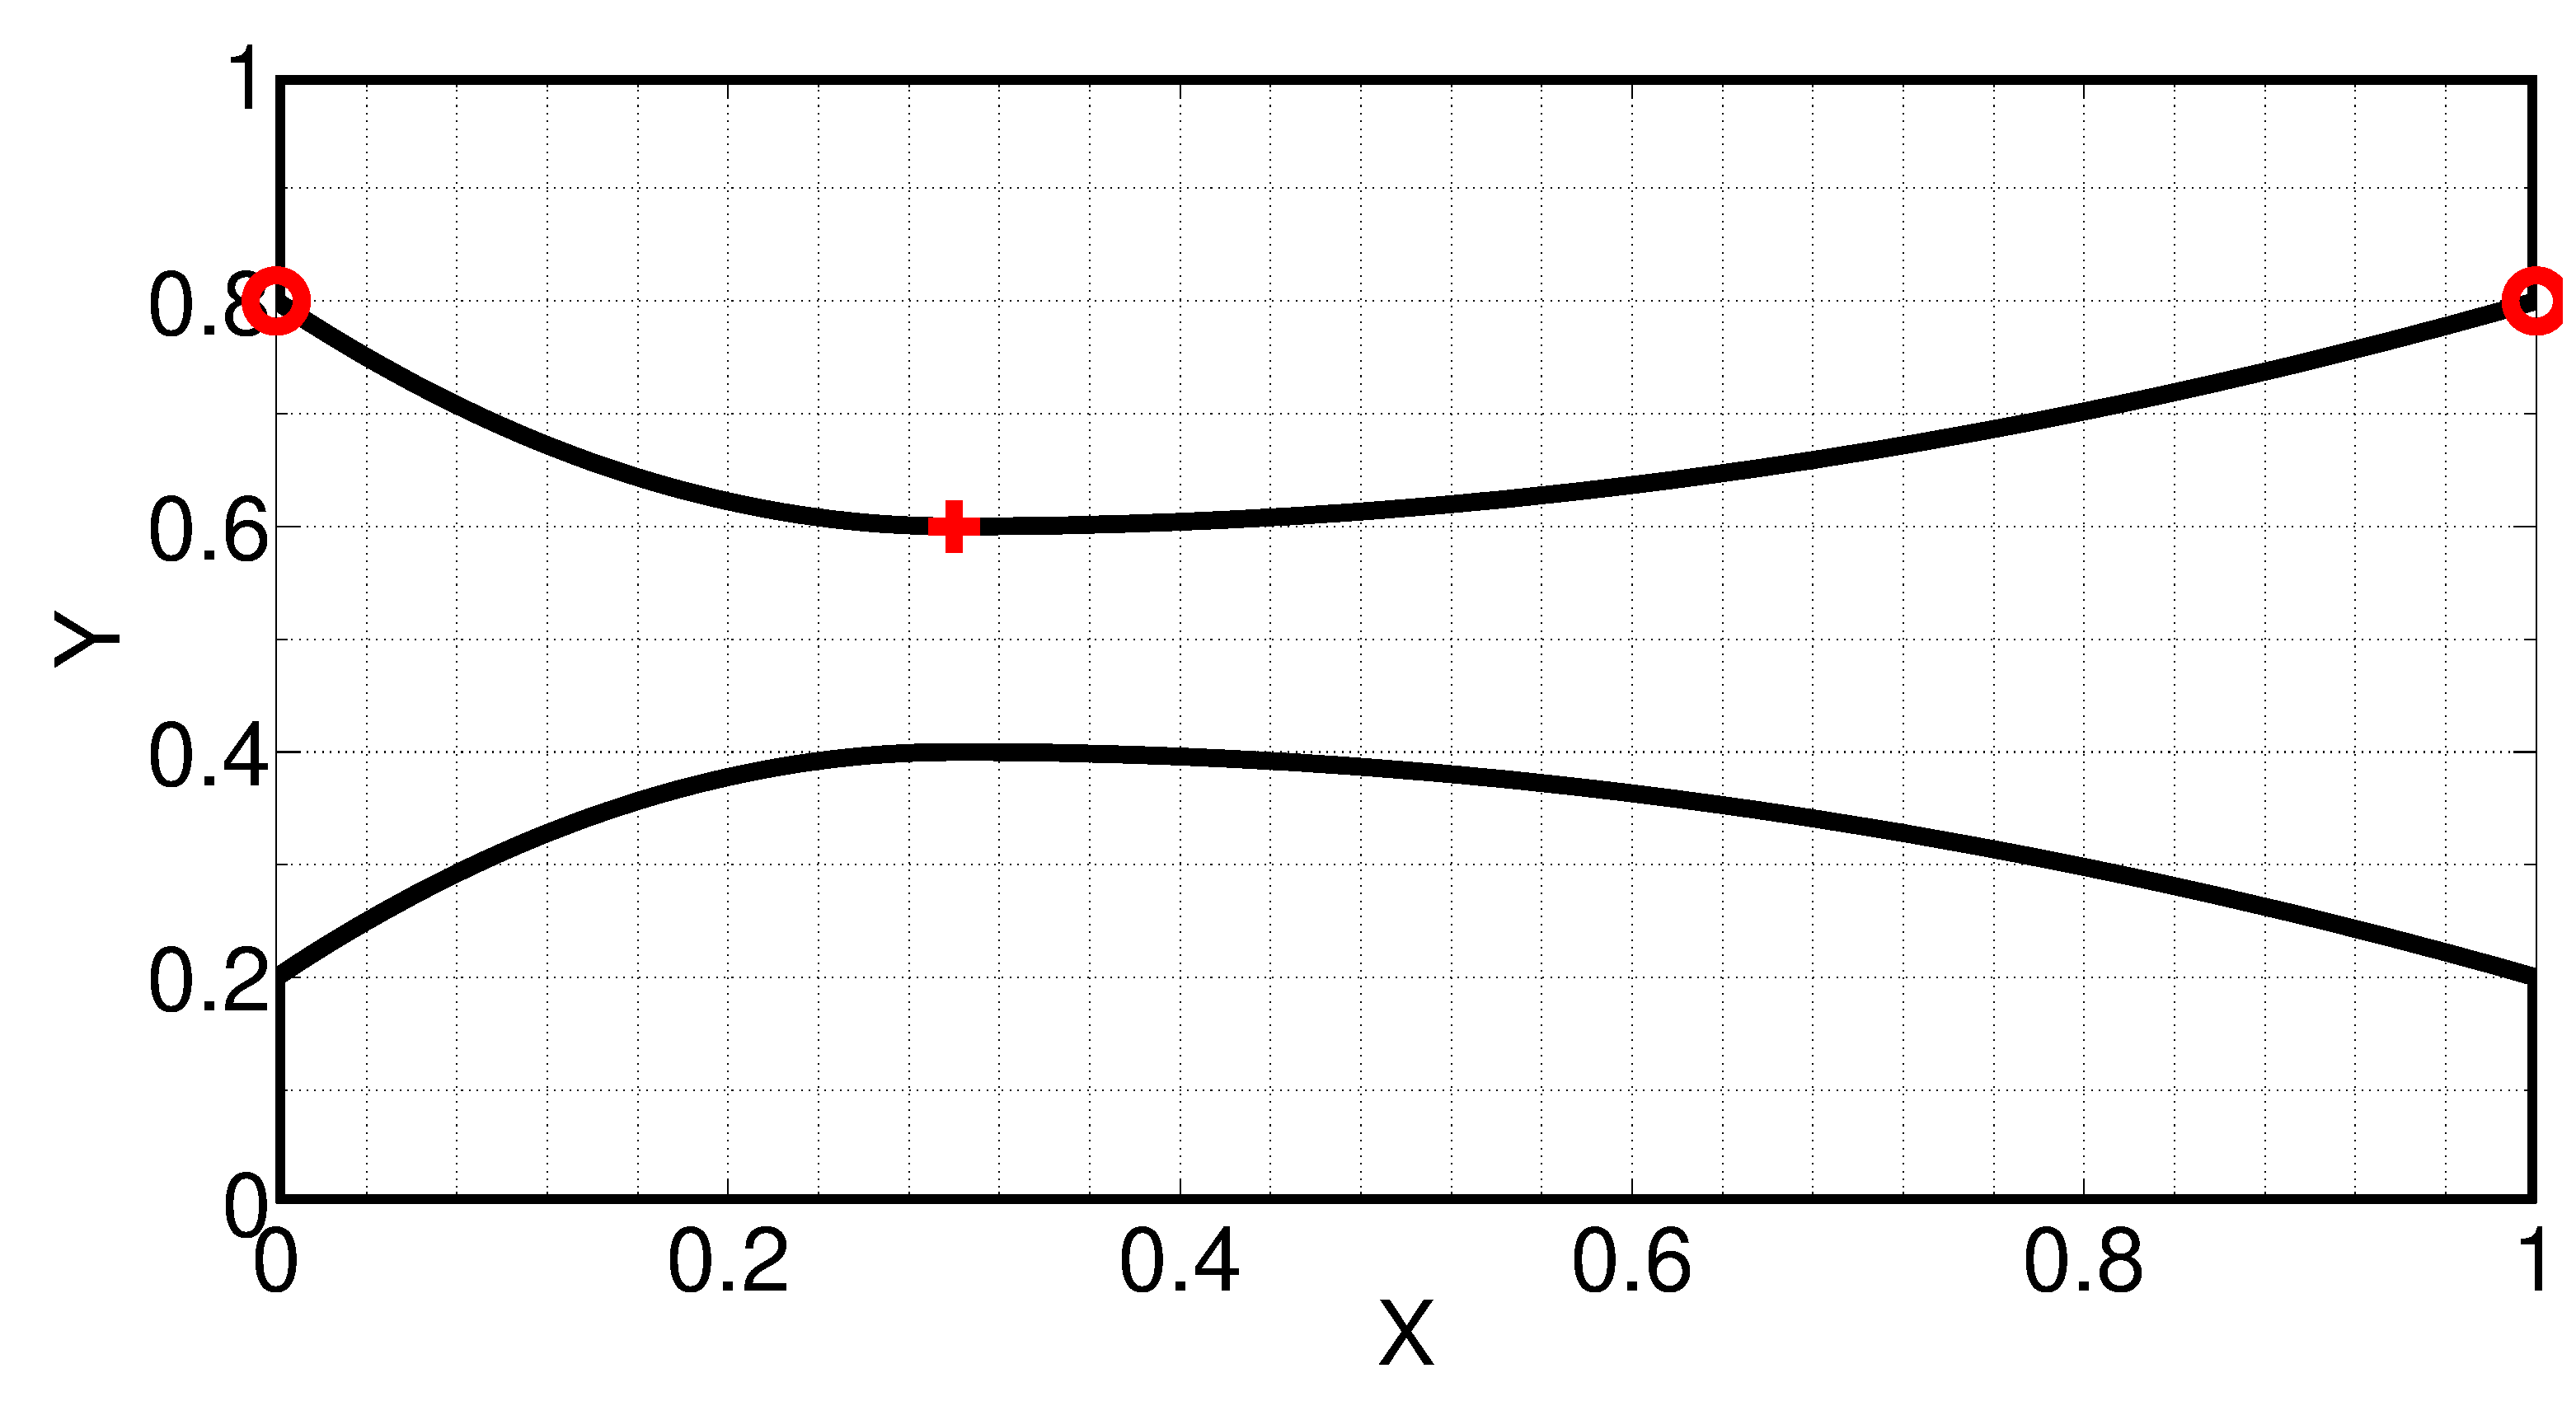
\includegraphics[width=7.0cm]{Chapter_4/figure/flow_through_nozzle/nozzle_shape_yt01.eps}
    }
    \quad
    \subfigure[Nozzle shape for $y_t = 0.2$]
    {
    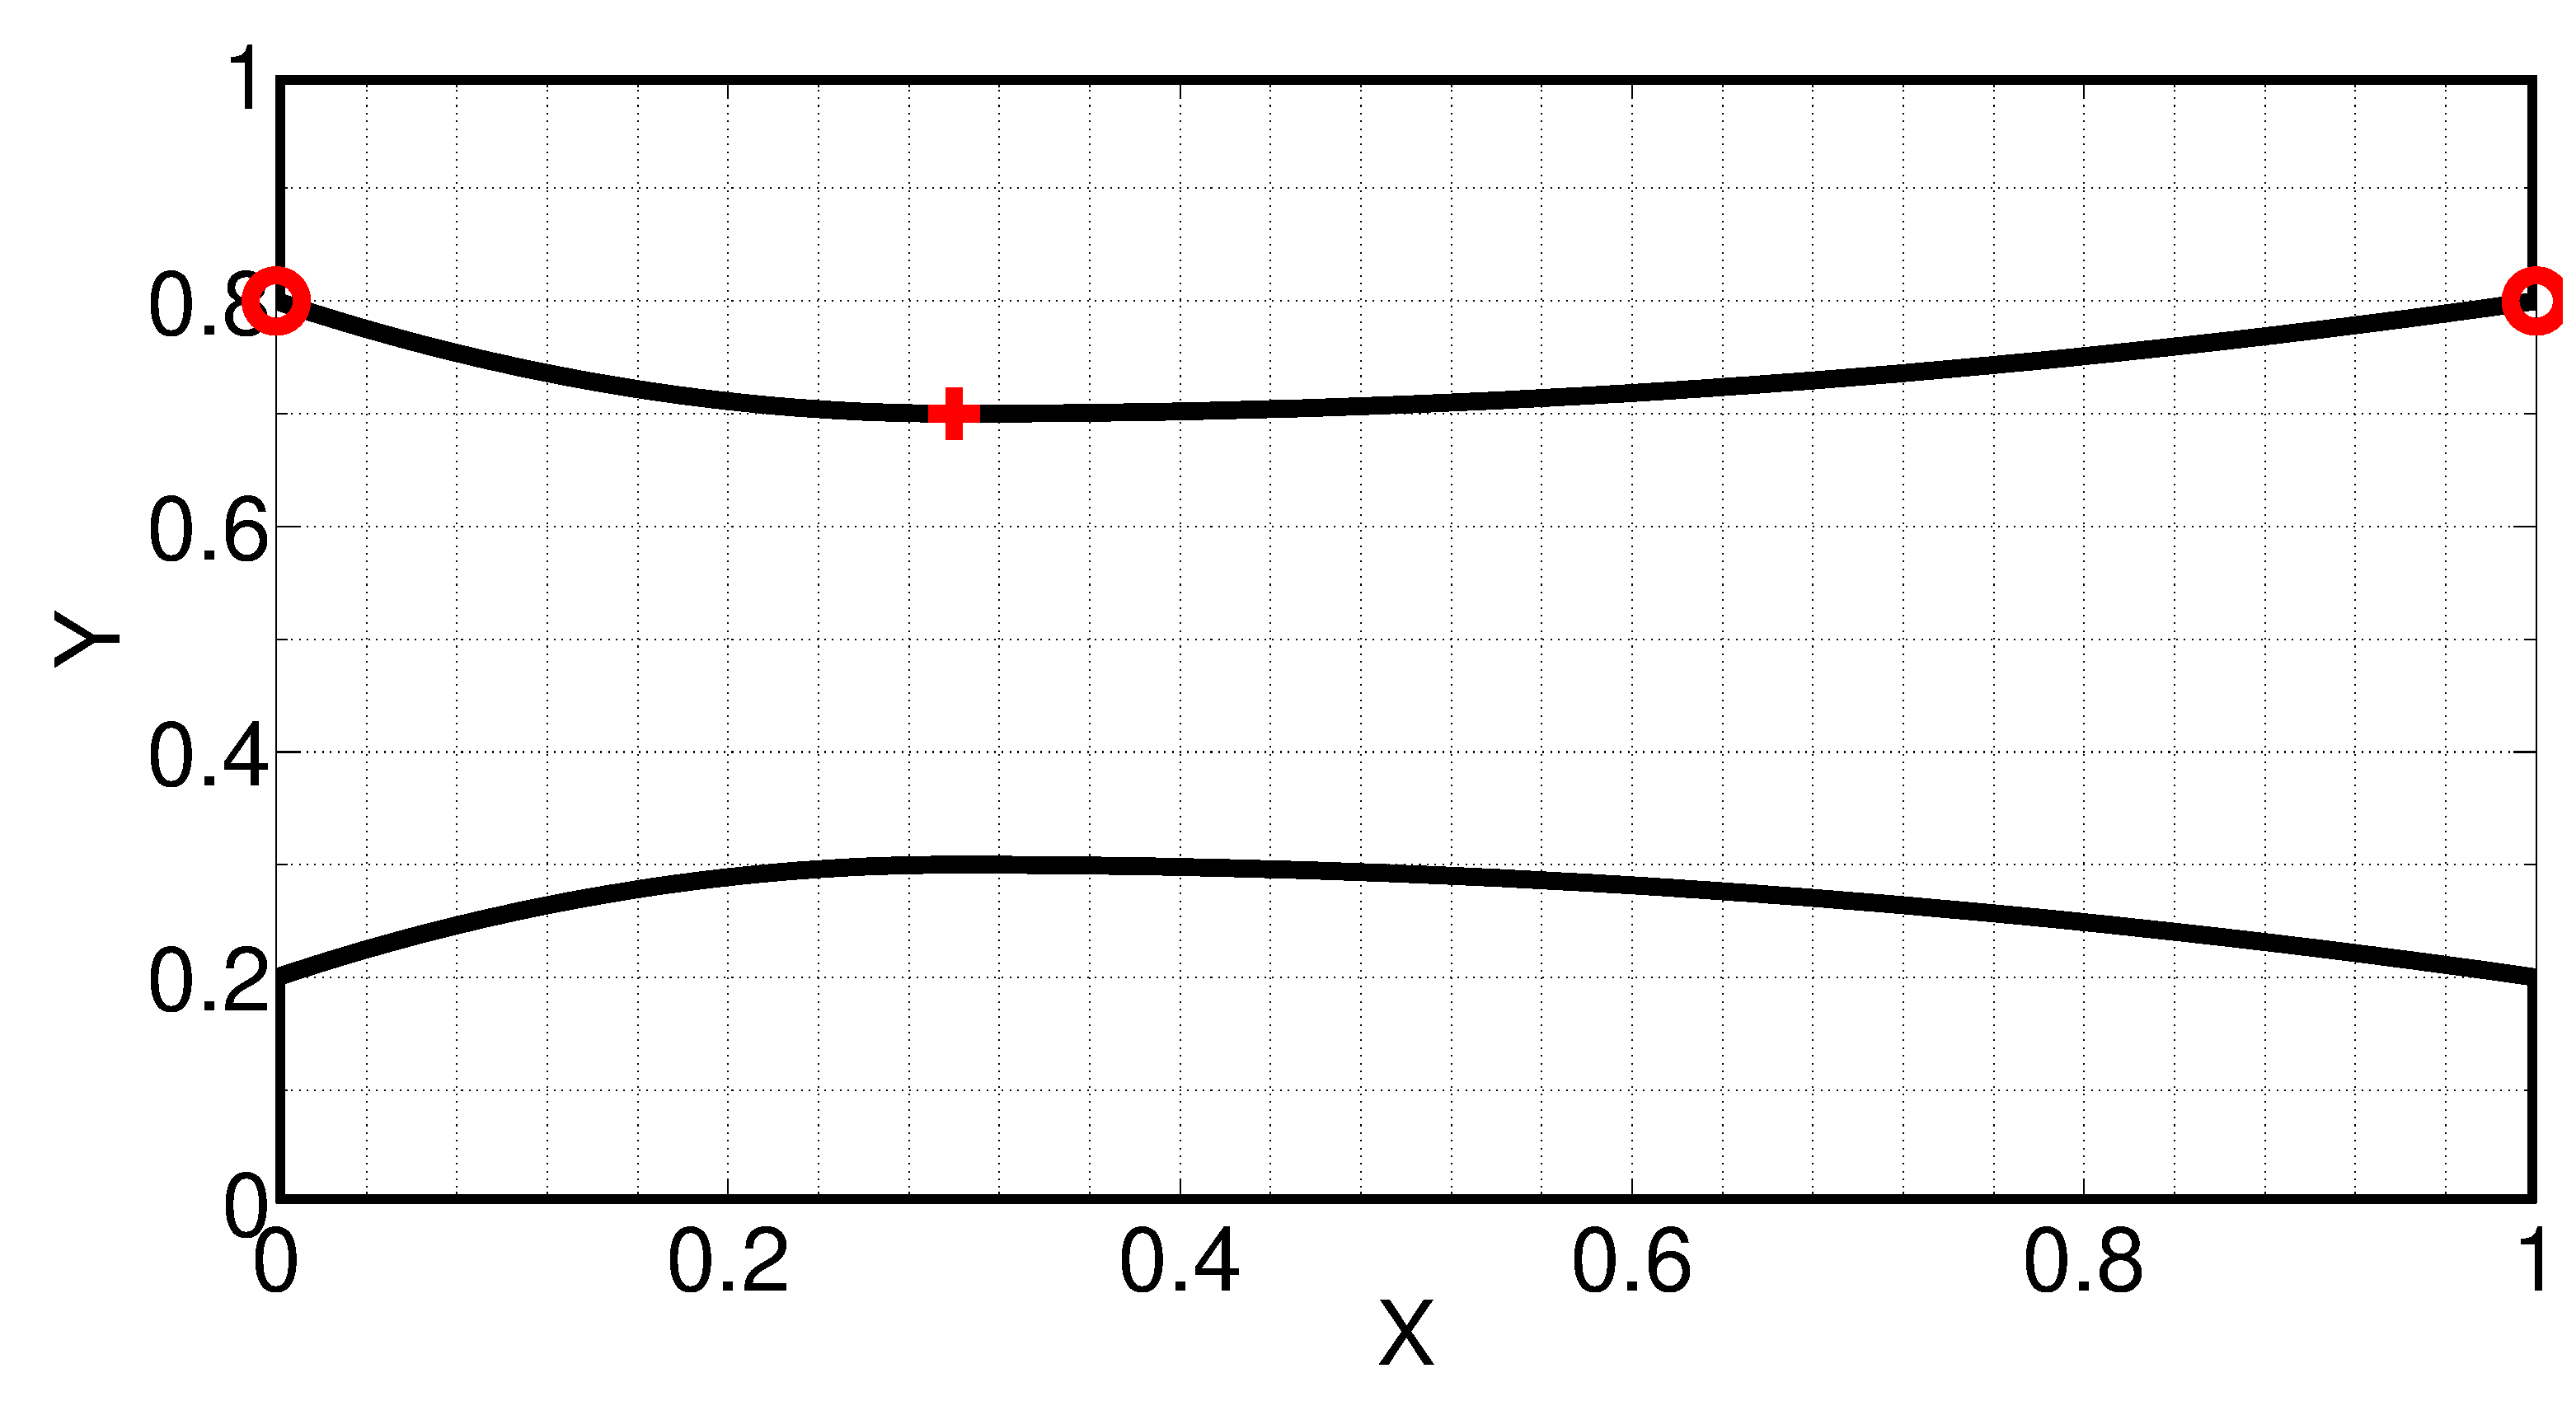
\includegraphics[width=7.0cm]{Chapter_4/figure/flow_through_nozzle/nozzle_shape_yt02.eps}
    }
    \caption{Effect of design variable on the shape of the nozzle.}
    \label{fig:C4_nozzleShape}
\end{figure}

The mesh convergence plots for the governing equations are shown in Figure \ref{fig:C4_nozzleFlow_meshConvergence}. As shown here, the mesh size of $500 \times 125$ is selected for the analysis.

\begin{figure}[H]
    \centering
    \subfigure[U-velocity mesh convergence.]
    {
    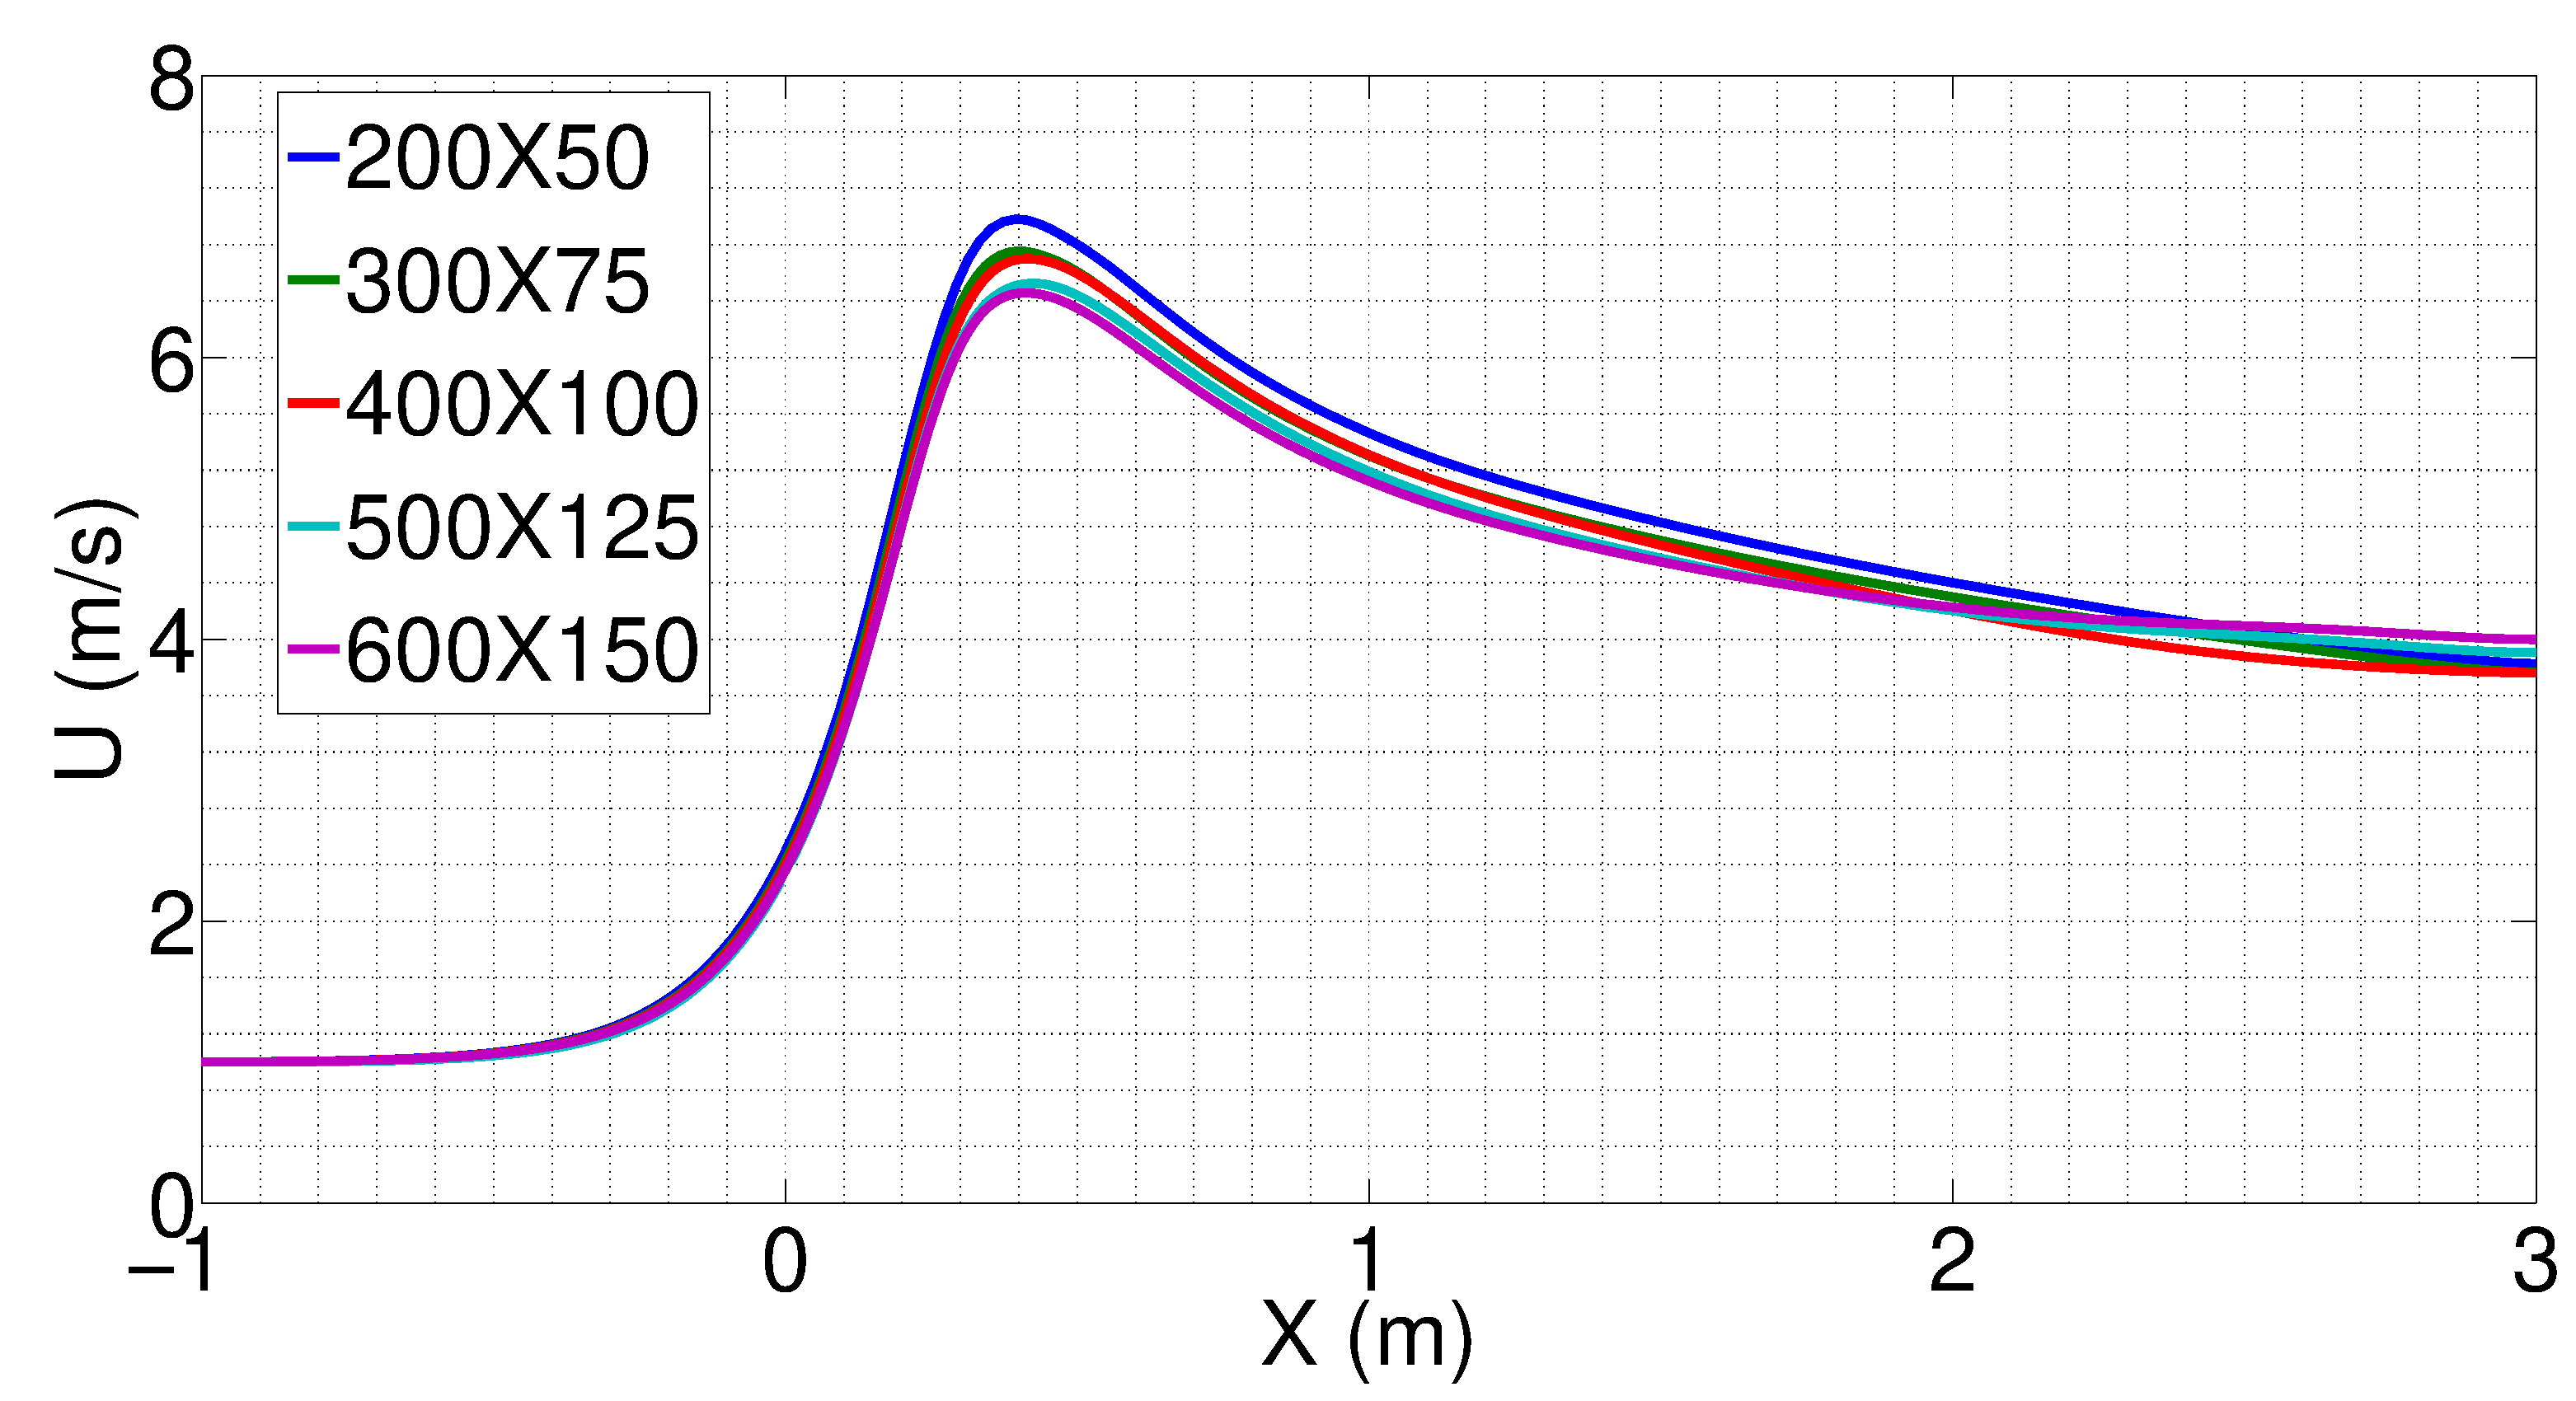
\includegraphics[width=7.0cm]{Chapter_4/figure/flow_through_nozzle/convergence_U_RE100.eps}
    }
    \quad
    \subfigure[V-velocity mesh convergence.]
    {
    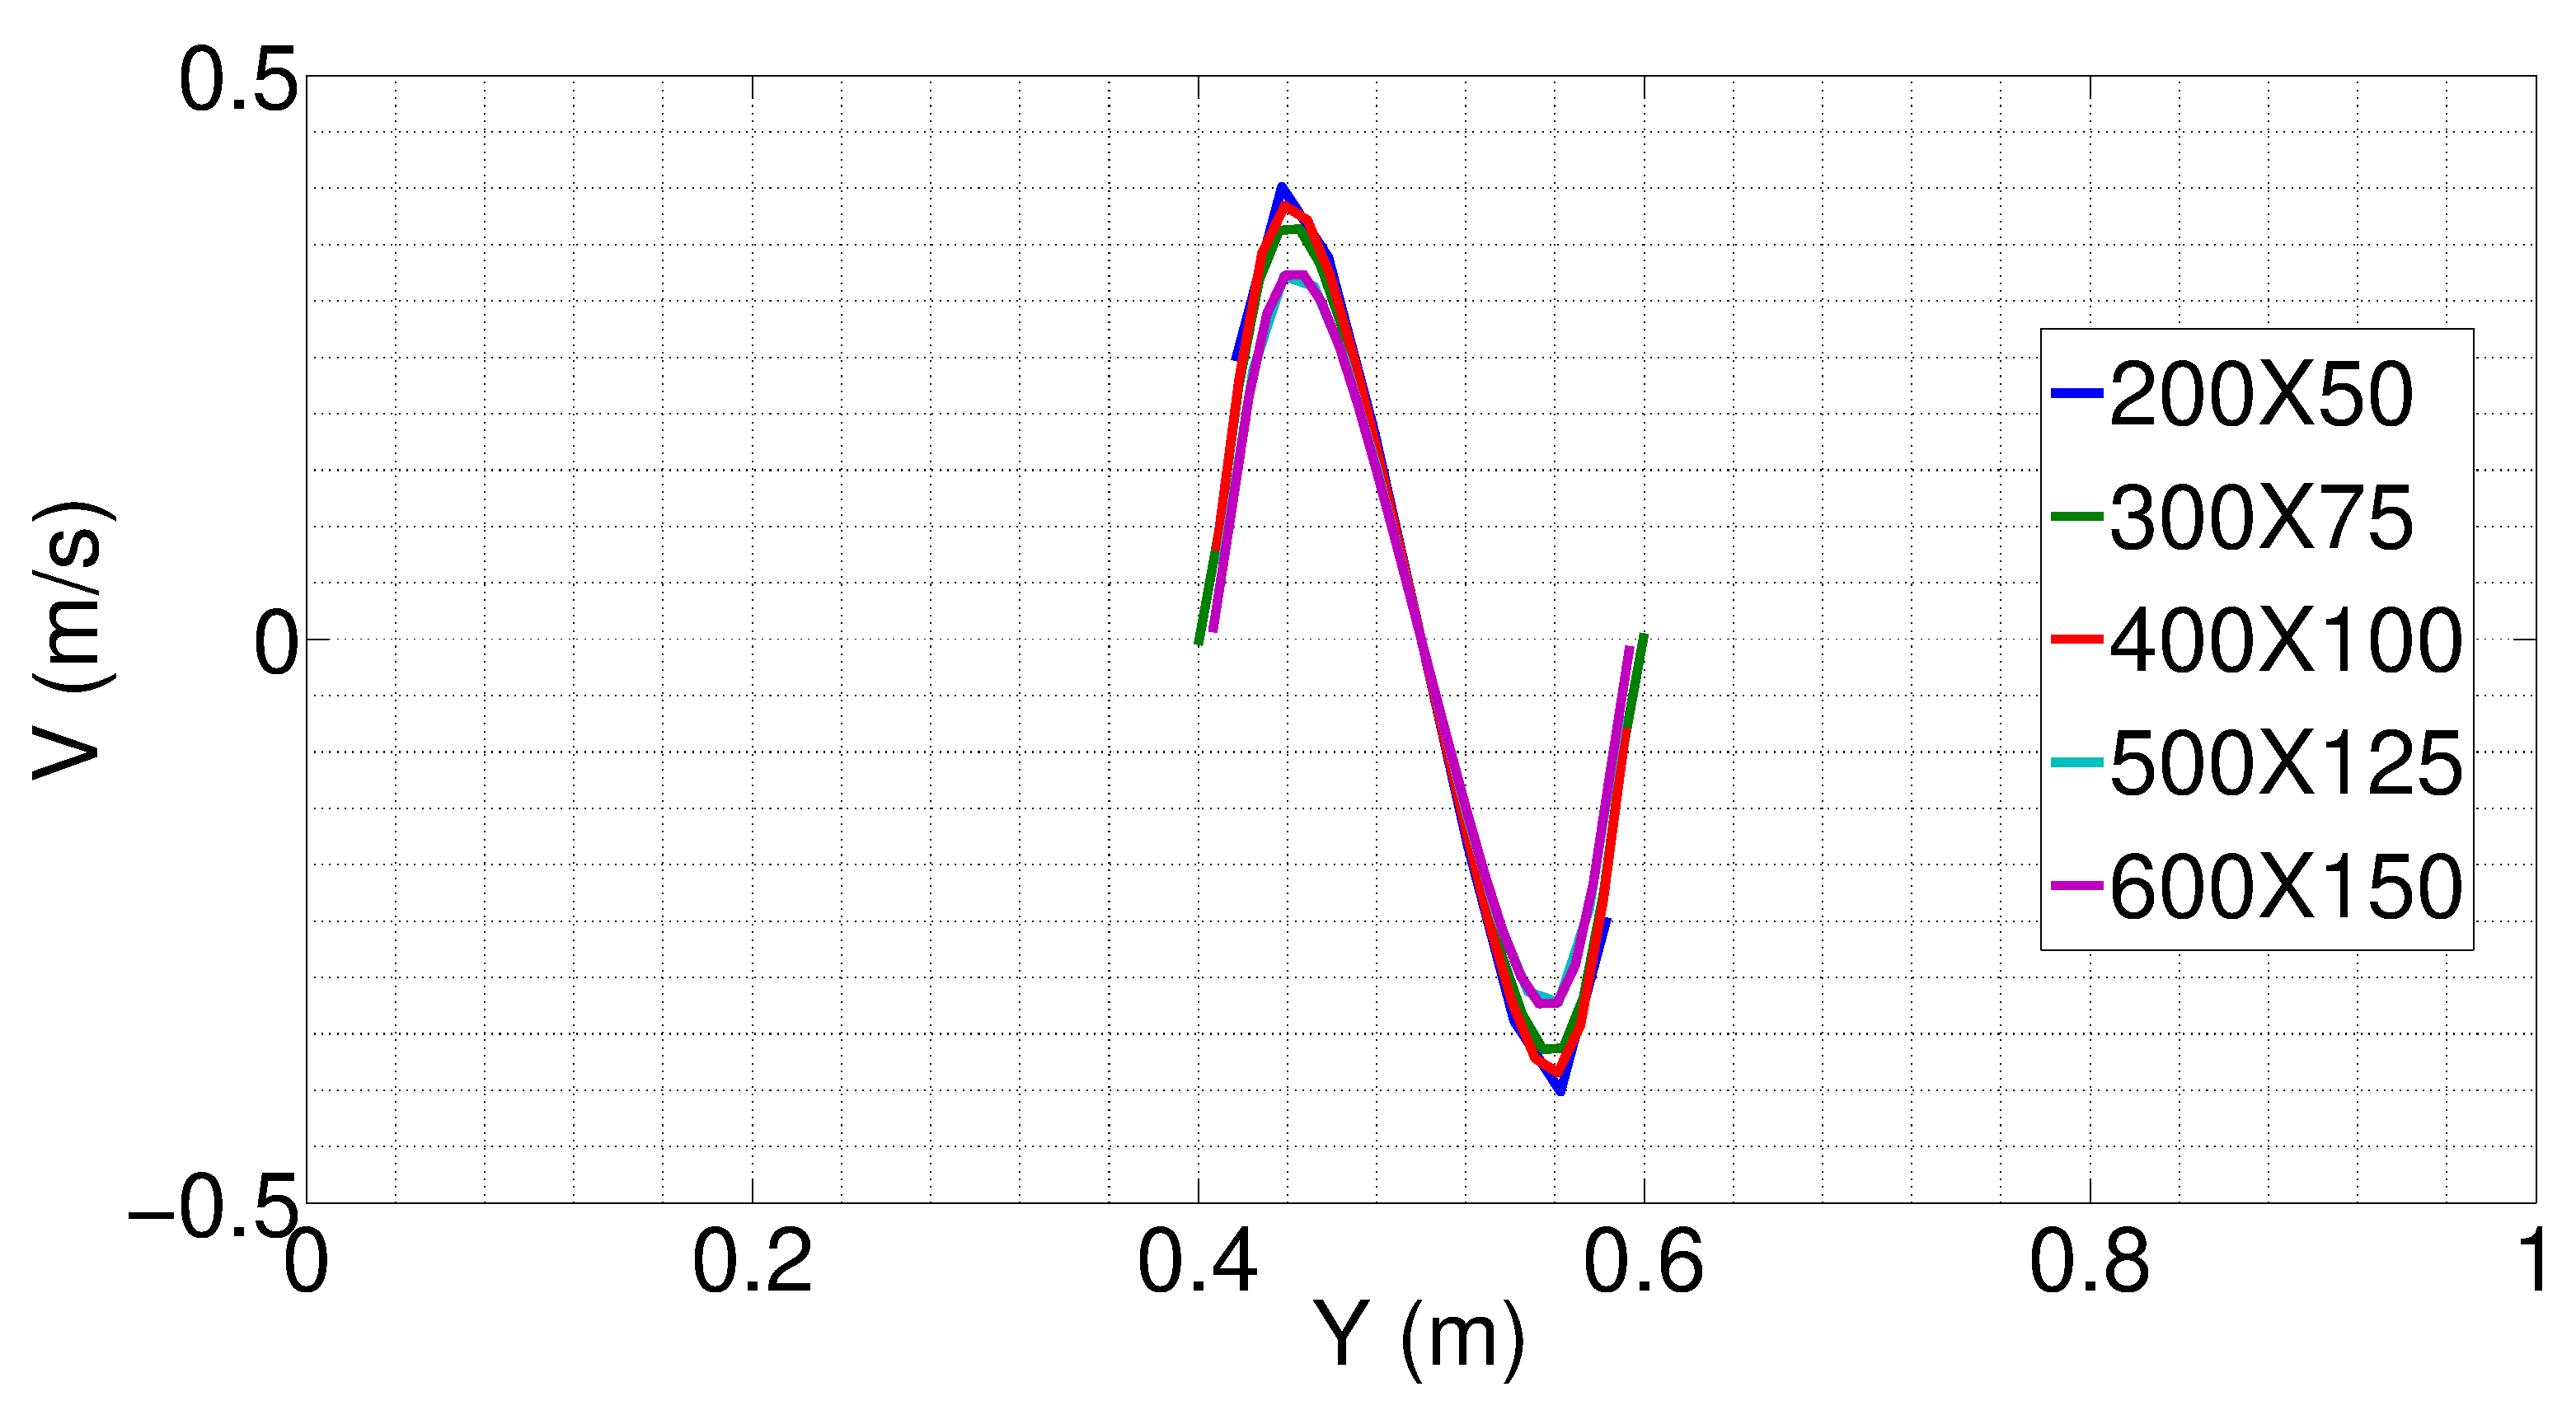
\includegraphics[width=7.0cm]{Chapter_4/figure/flow_through_nozzle/convergence_V_RE100.eps}
    }
    \\
    \subfigure[Pressure mesh convergence.]
    {
    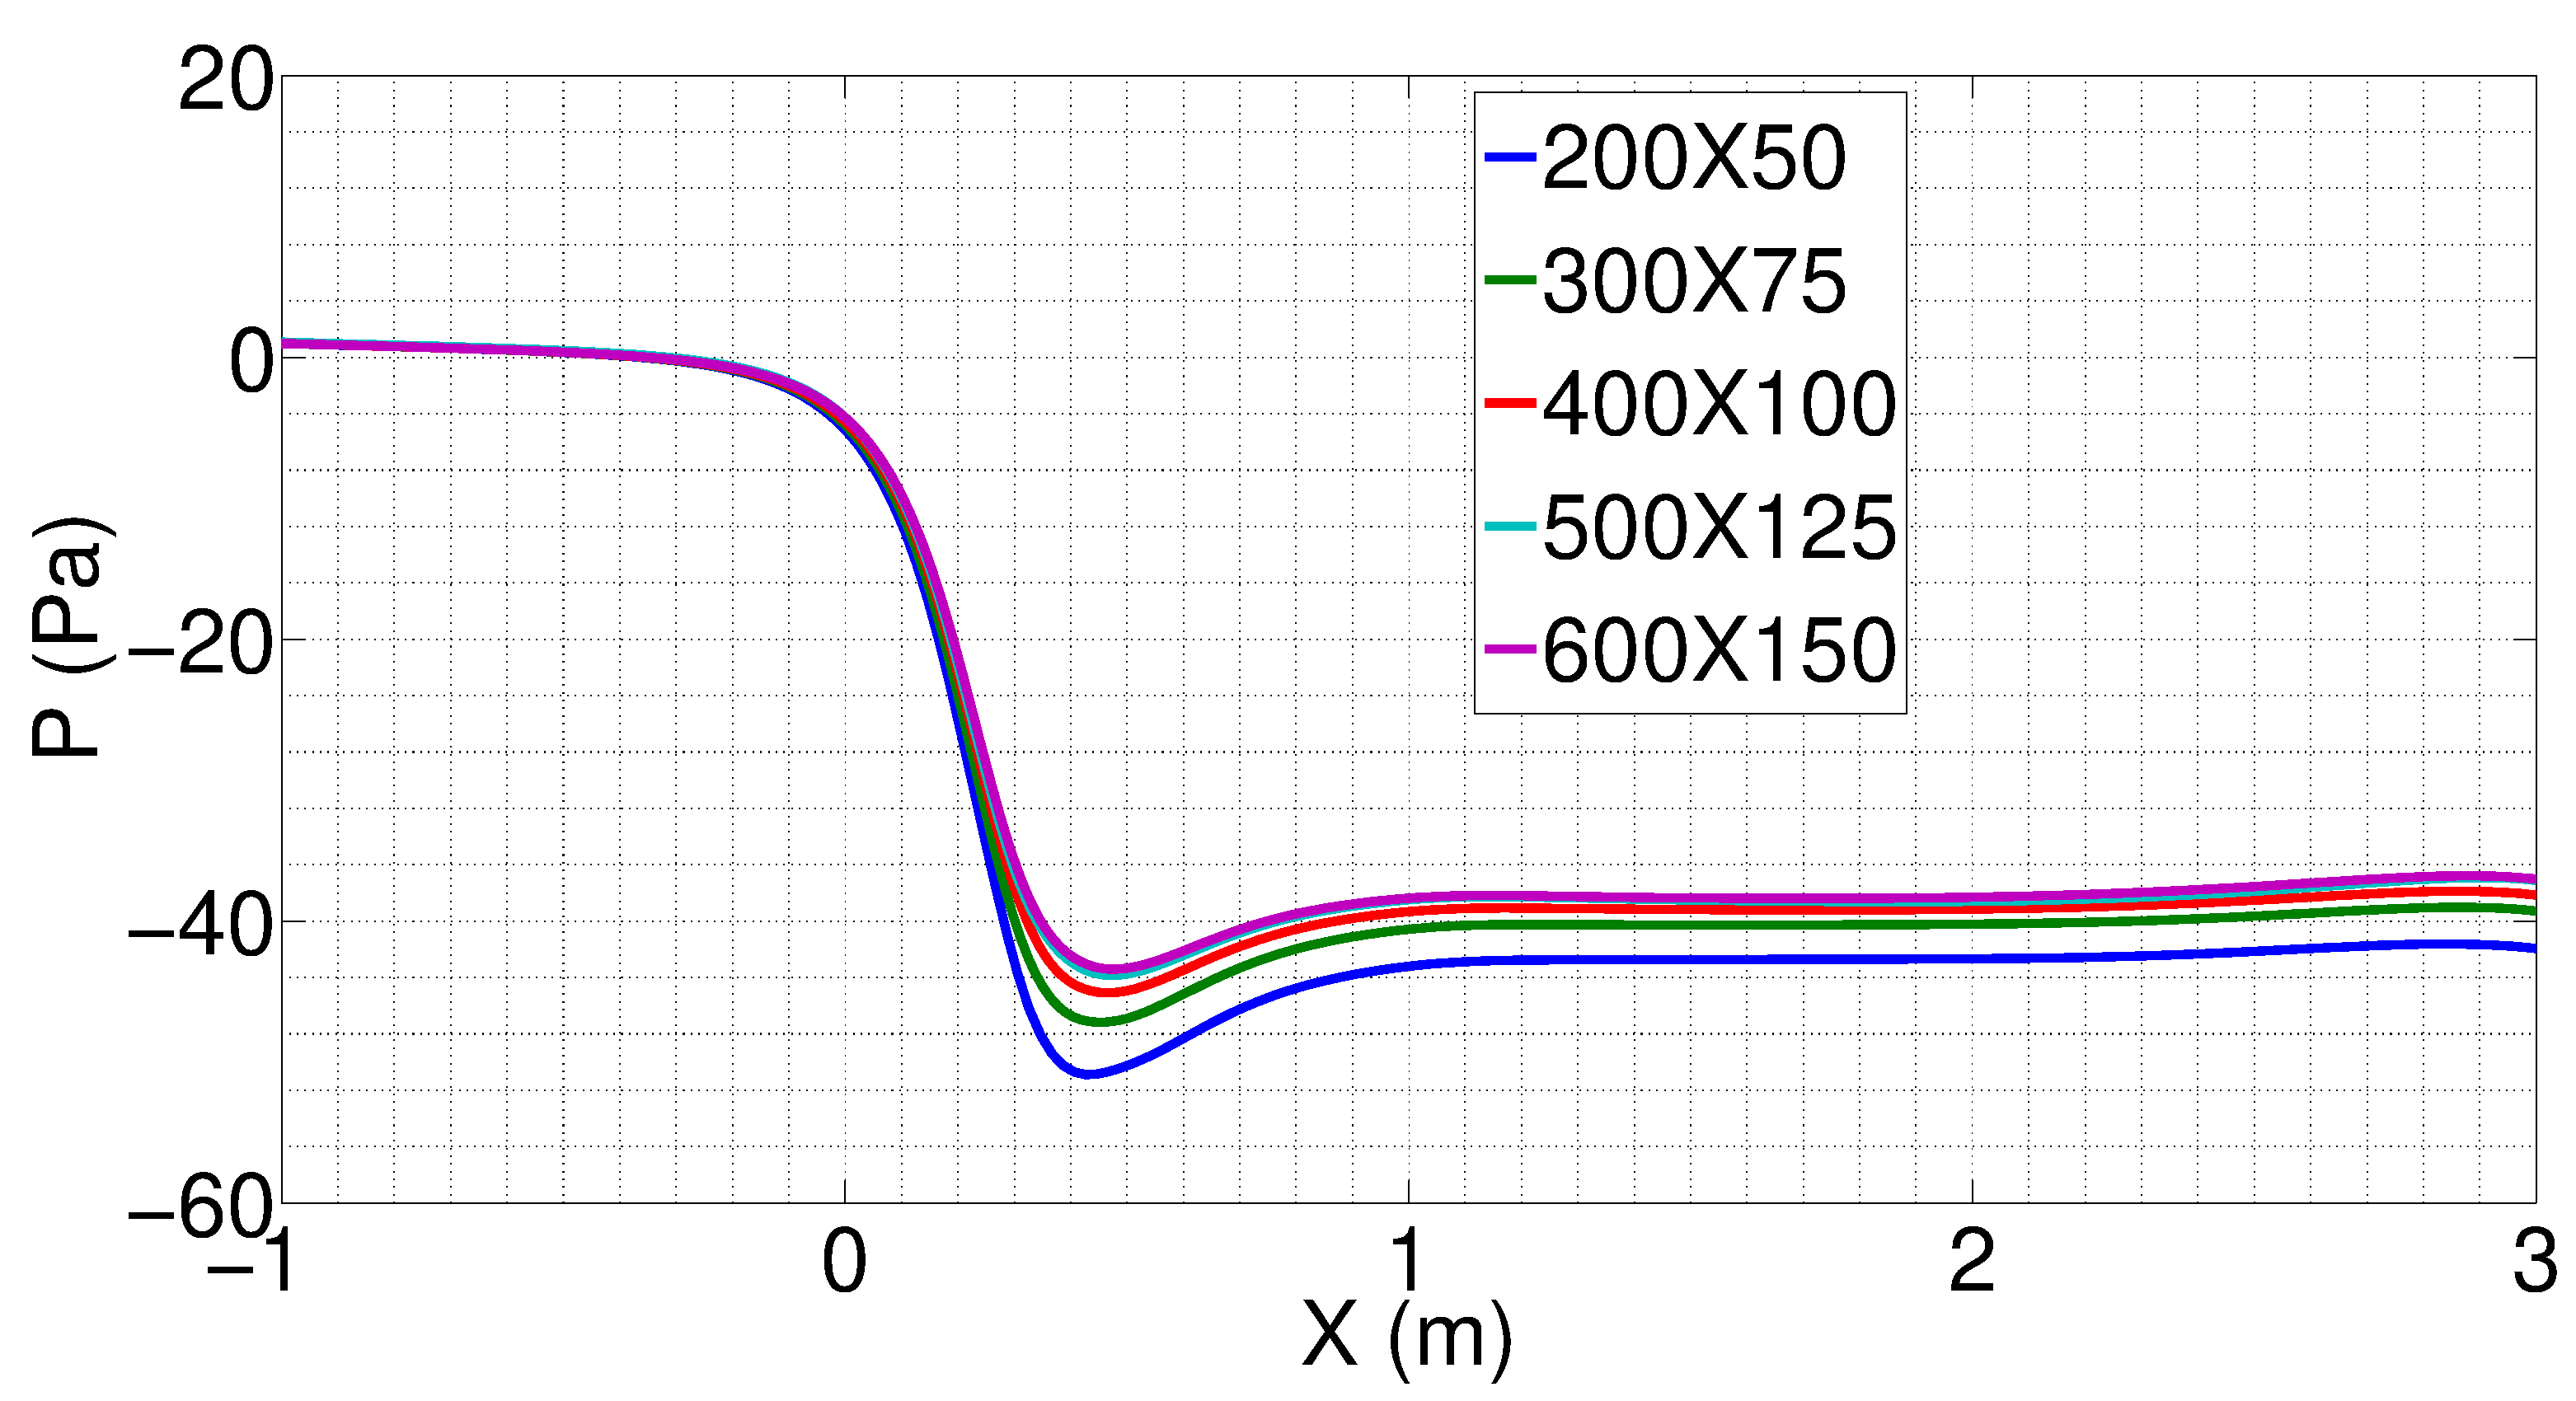
\includegraphics[width=7.0cm]{Chapter_4/figure/flow_through_nozzle/convergence_P_RE100.eps}
    }
    \caption{Mesh convergence study for the governing equation.}
    \label{fig:C4_nozzleFlow_meshConvergence}
\end{figure}

The convergence rate is shown in Figure \ref{fig:C4_nozzleFlow_meshConvergenceRate}. A mesh node at the throat area on the symmetry line is selected for this study for u-velocity and pressure. Since the v-velocity is zero for this point, a node at $(0.3, 0
.55)$ is selected for the convergence study of the v-velocity. The slope of the dotted line in Figure \ref{fig:C4_nozzleFlow_meshConvergenceRate} is calculated as $-0.96$, $-0.86$, and $-0.73$ for u-velocity, v-velocity, and pressure error, respectfully. The convergence is close to first order due to the relative location of the points to the solid walls where the approximation is first order.

\begin{figure}[H]
    \centering
    \subfigure[U-velocity convergence rate at $(0.3, 0.0)$.]
    {
    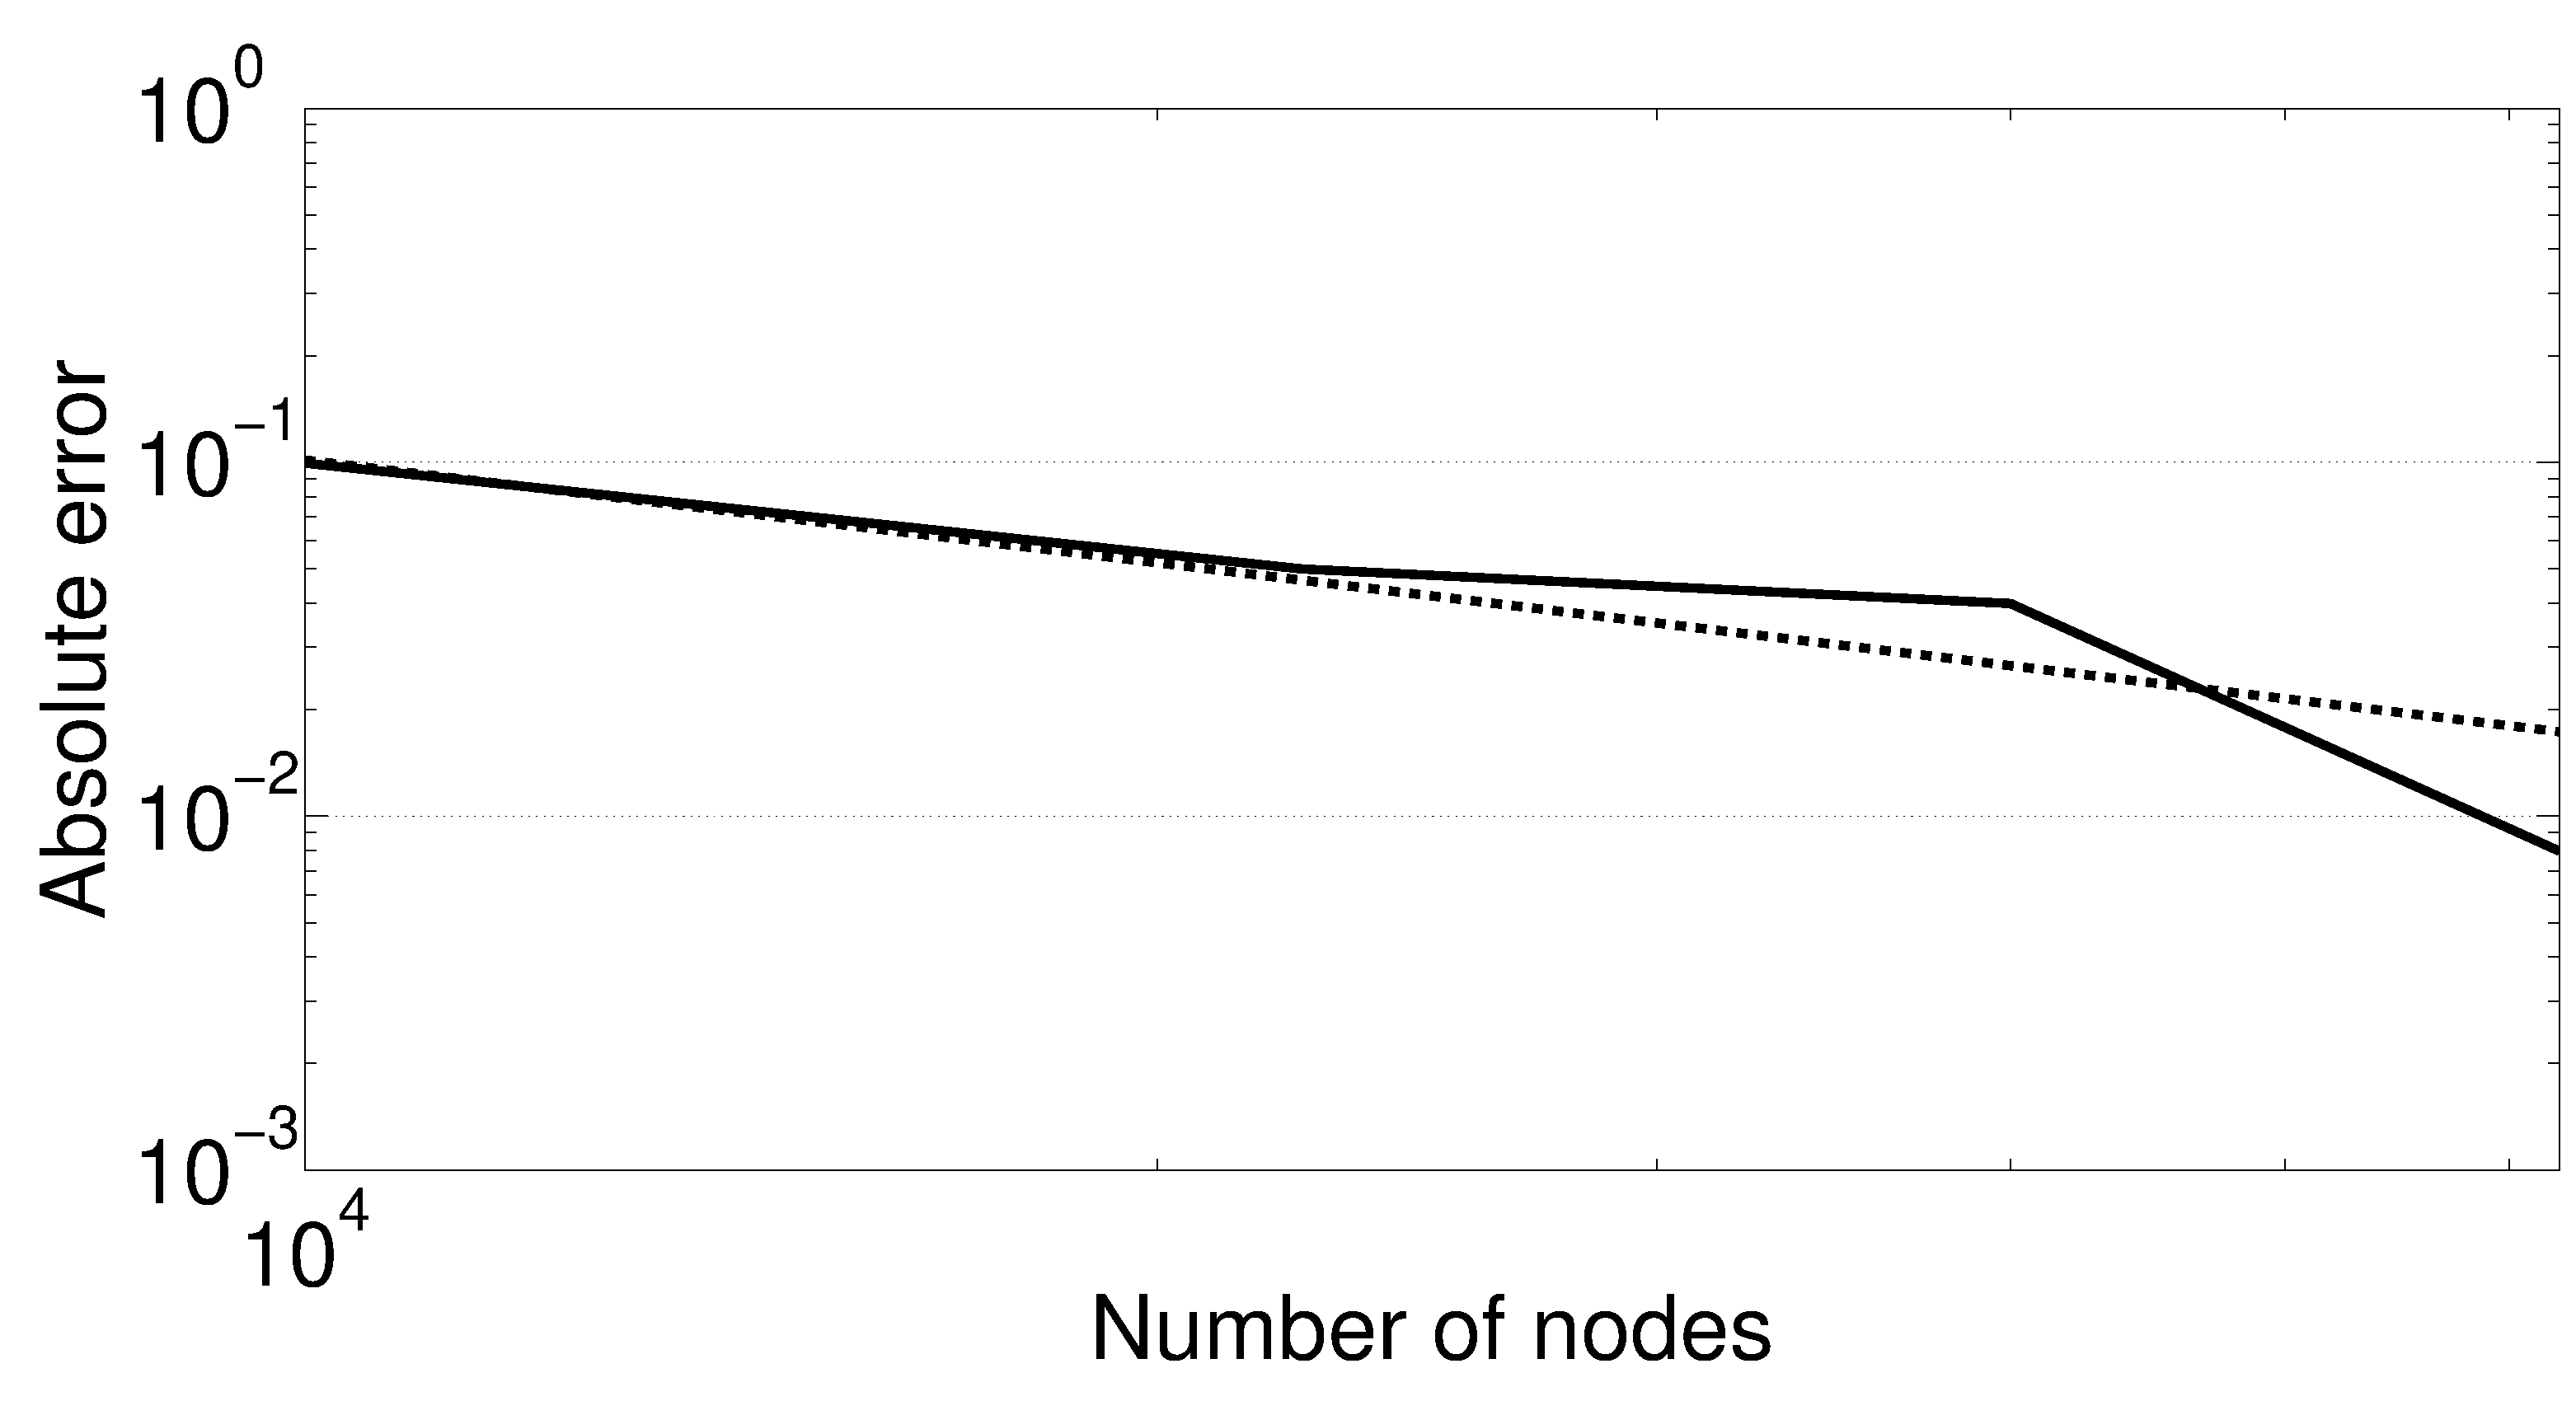
\includegraphics[width=7.0cm]{Chapter_4/figure/flow_through_nozzle/convergenceRate_U_RE100.eps}
    }
    \quad
    \subfigure[V-velocity convergence rate at $(0.3, 0.55)$.]
    {
    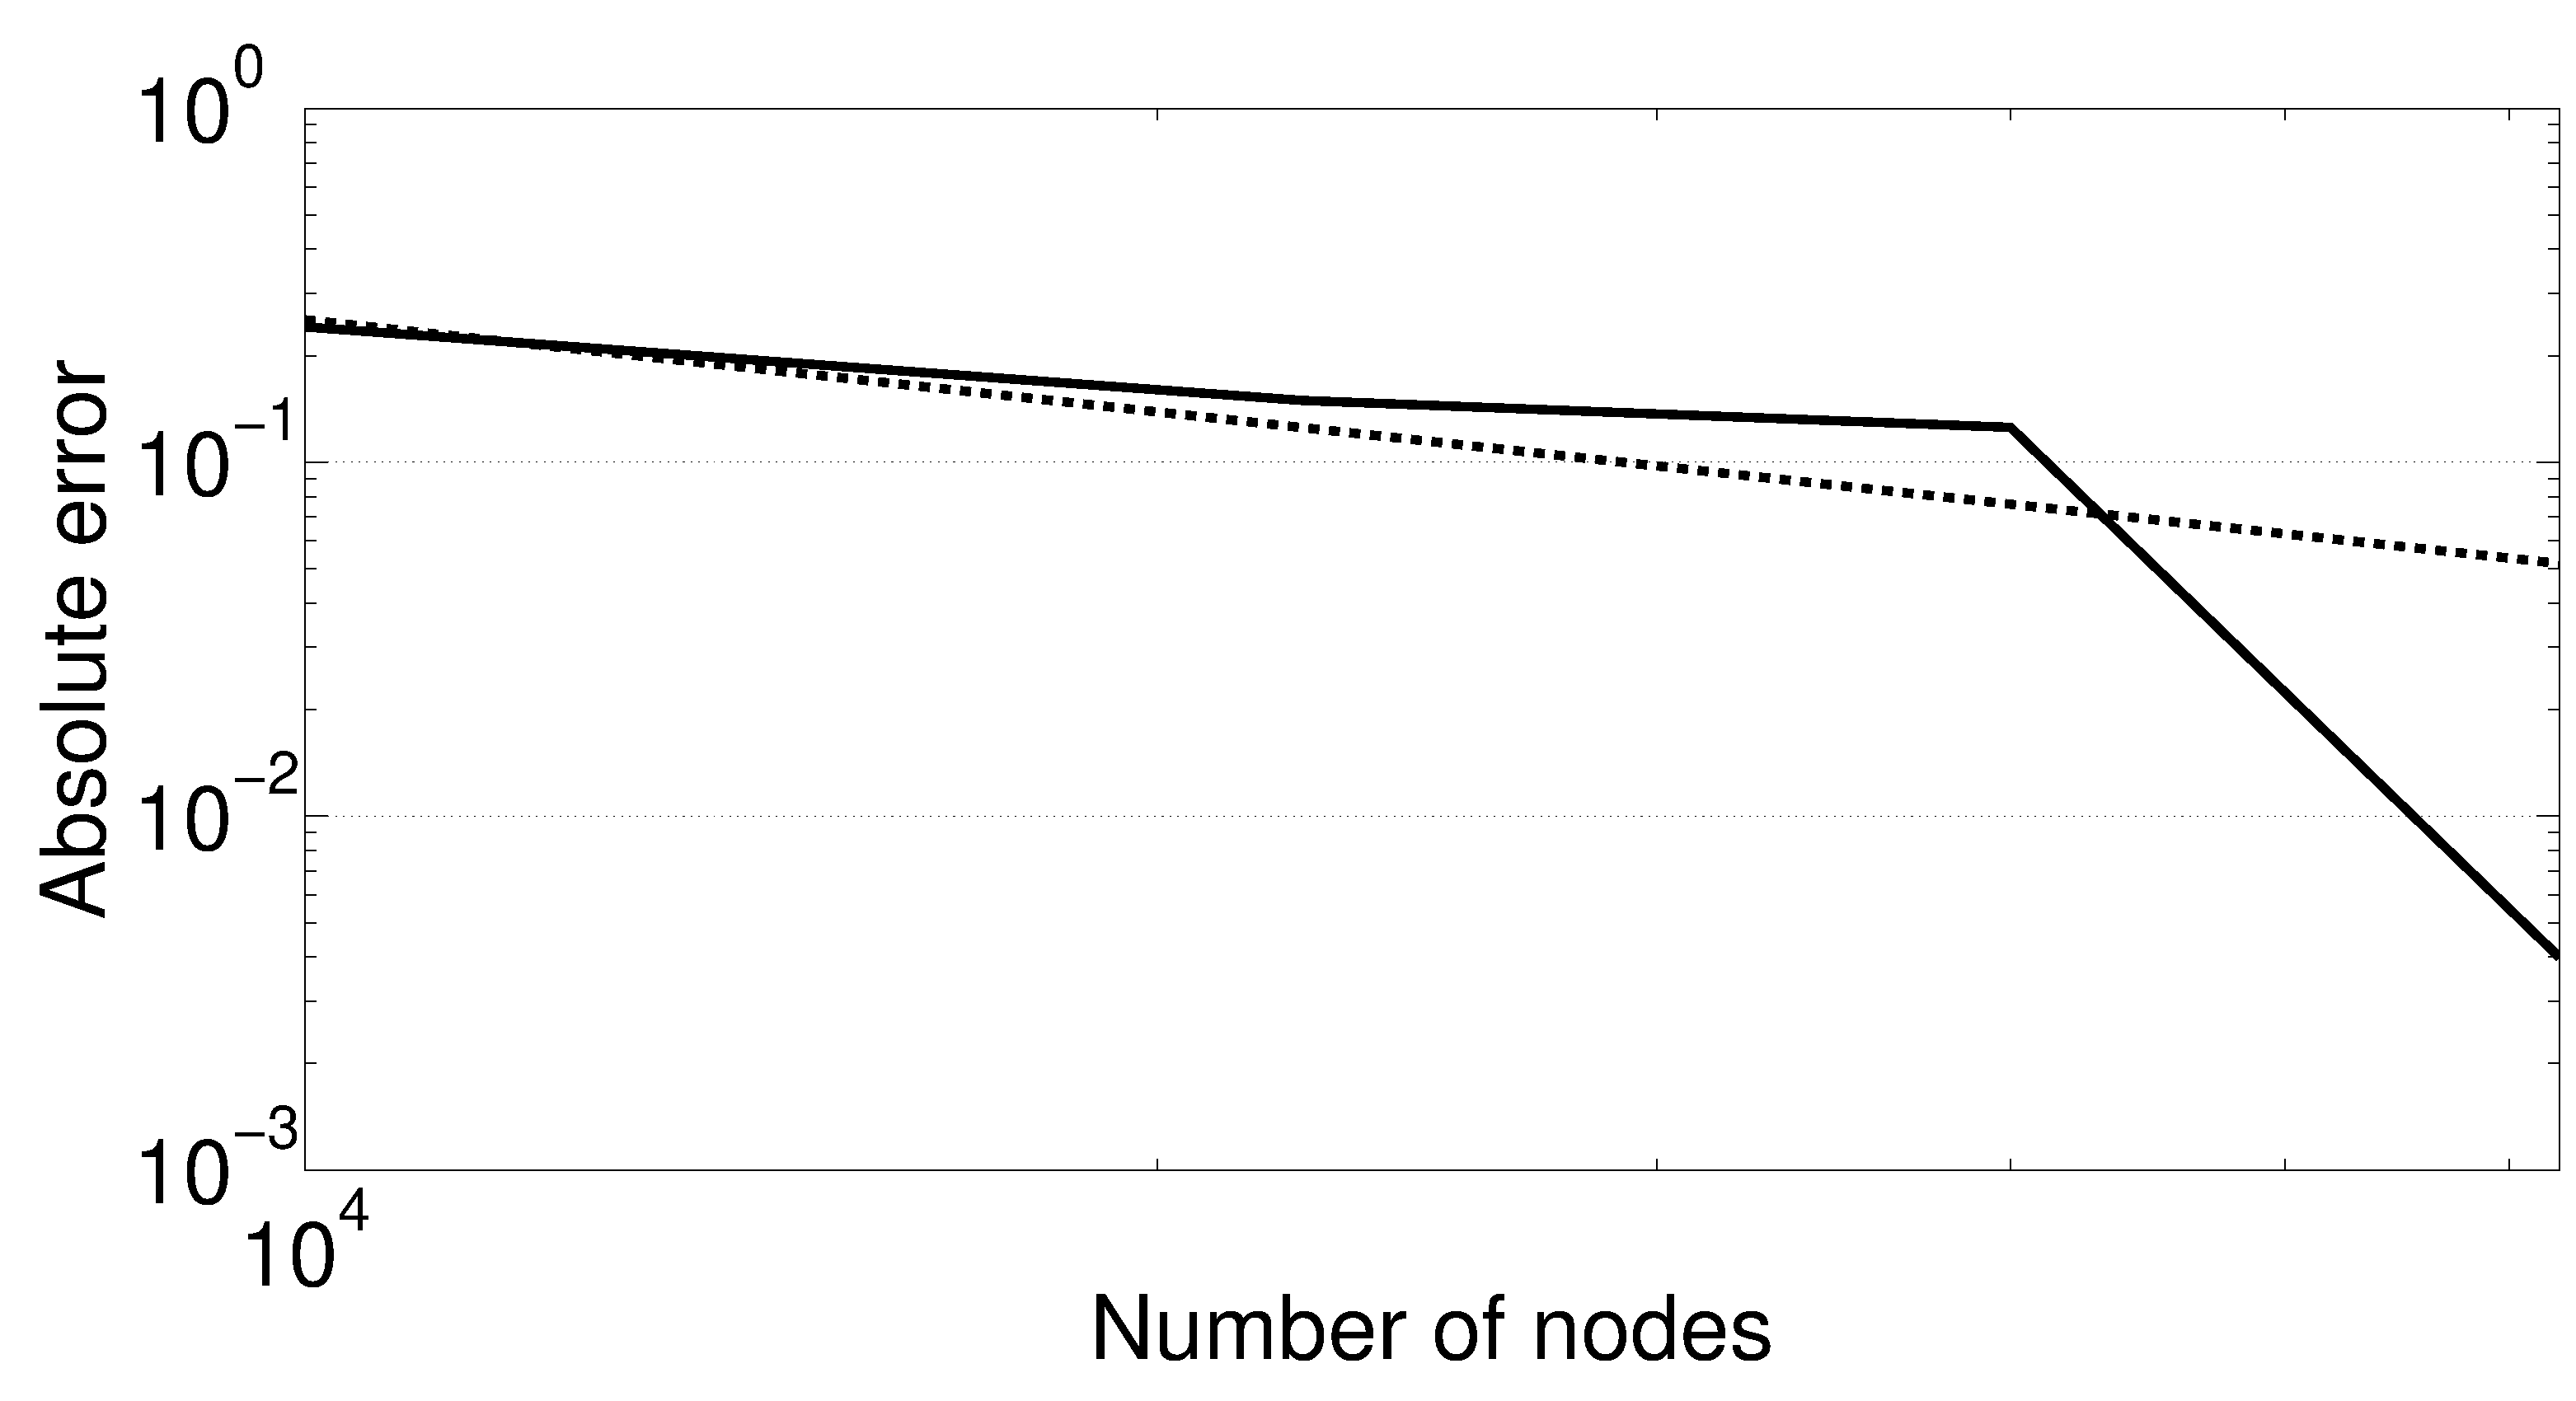
\includegraphics[width=7.0cm]{Chapter_4/figure/flow_through_nozzle/convergenceRate_V_RE100.eps}
    }
    \\
    \subfigure[Pressure  convergence rate at $(0.3, 0.0)$..]
    {
    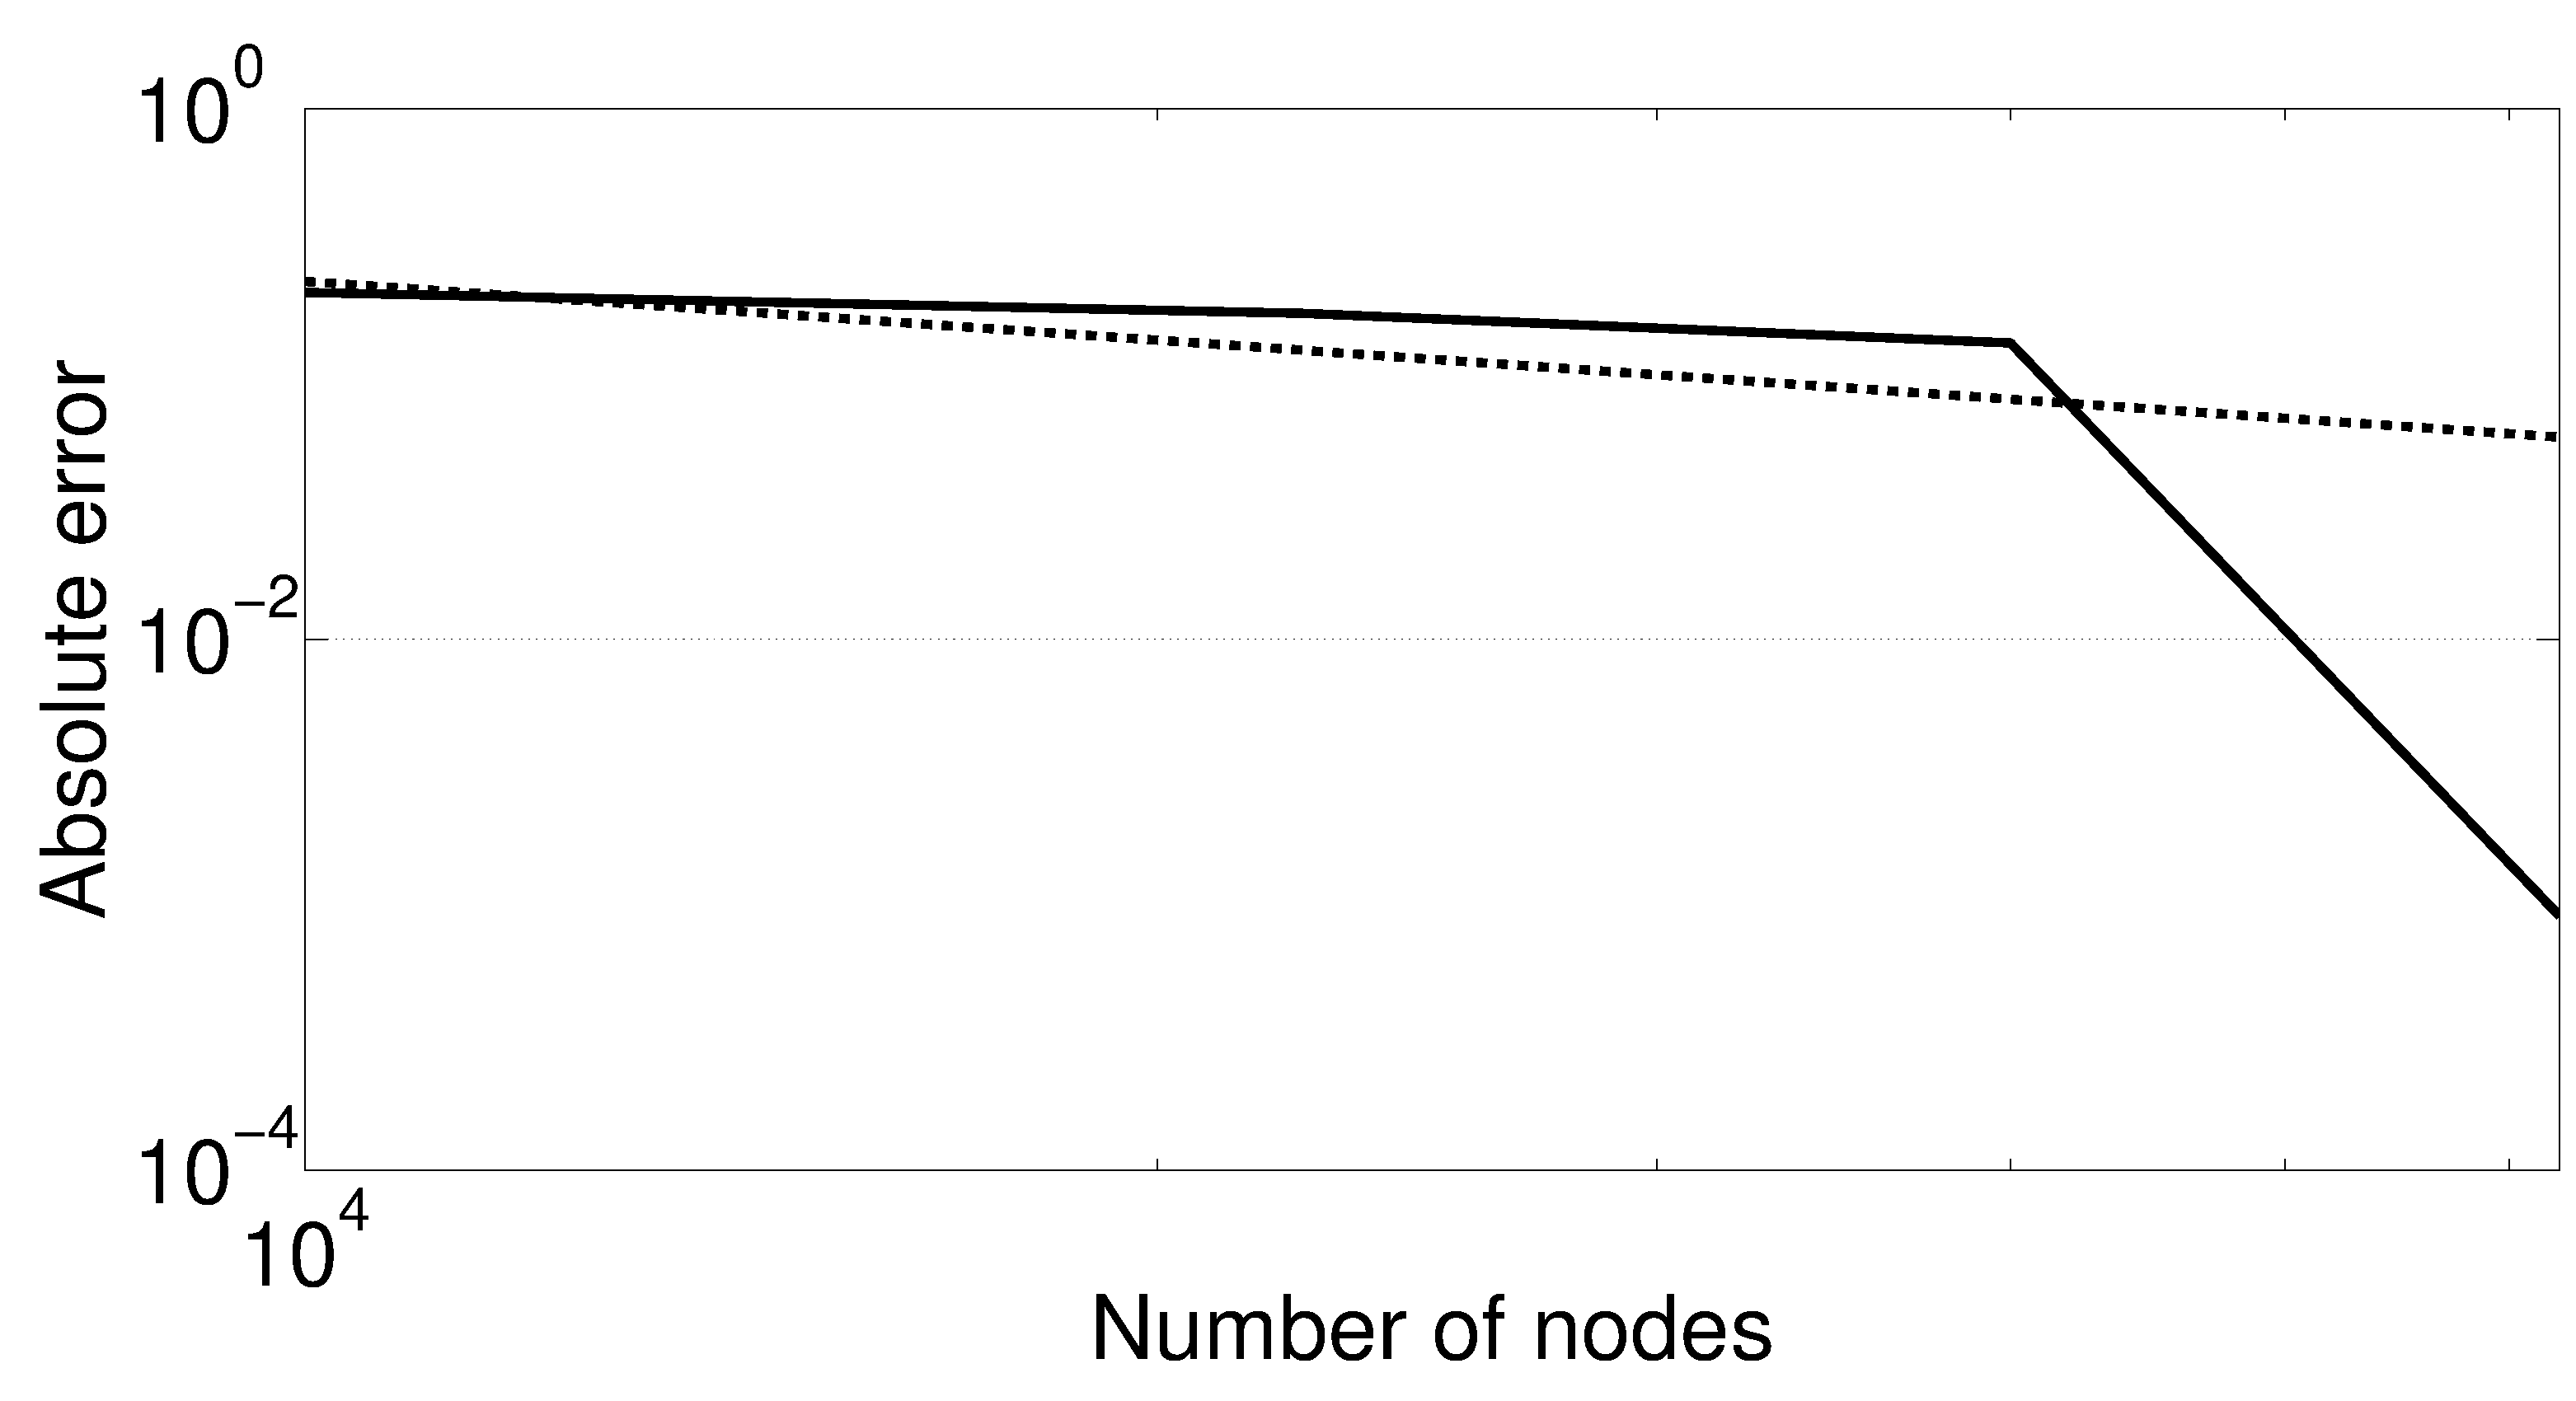
\includegraphics[width=7.0cm]{Chapter_4/figure/flow_through_nozzle/convergenceRate_P_RE100.eps}
    }
    \caption{Mesh convergence study for the governing equation.}
    \label{fig:C4_nozzleFlow_meshConvergenceRate}
\end{figure}

The contour plots for the velocities through the nozzle are shown in Figure \ref{fig:C4_nozzleFlow_contourForAnalysis}. As shown here, the forcing function was able to model the walls and cause the flow to accelerate through the nozzle.

\begin{figure}[H]
    \centering
    \subfigure[U-velocity contour.]
    {
    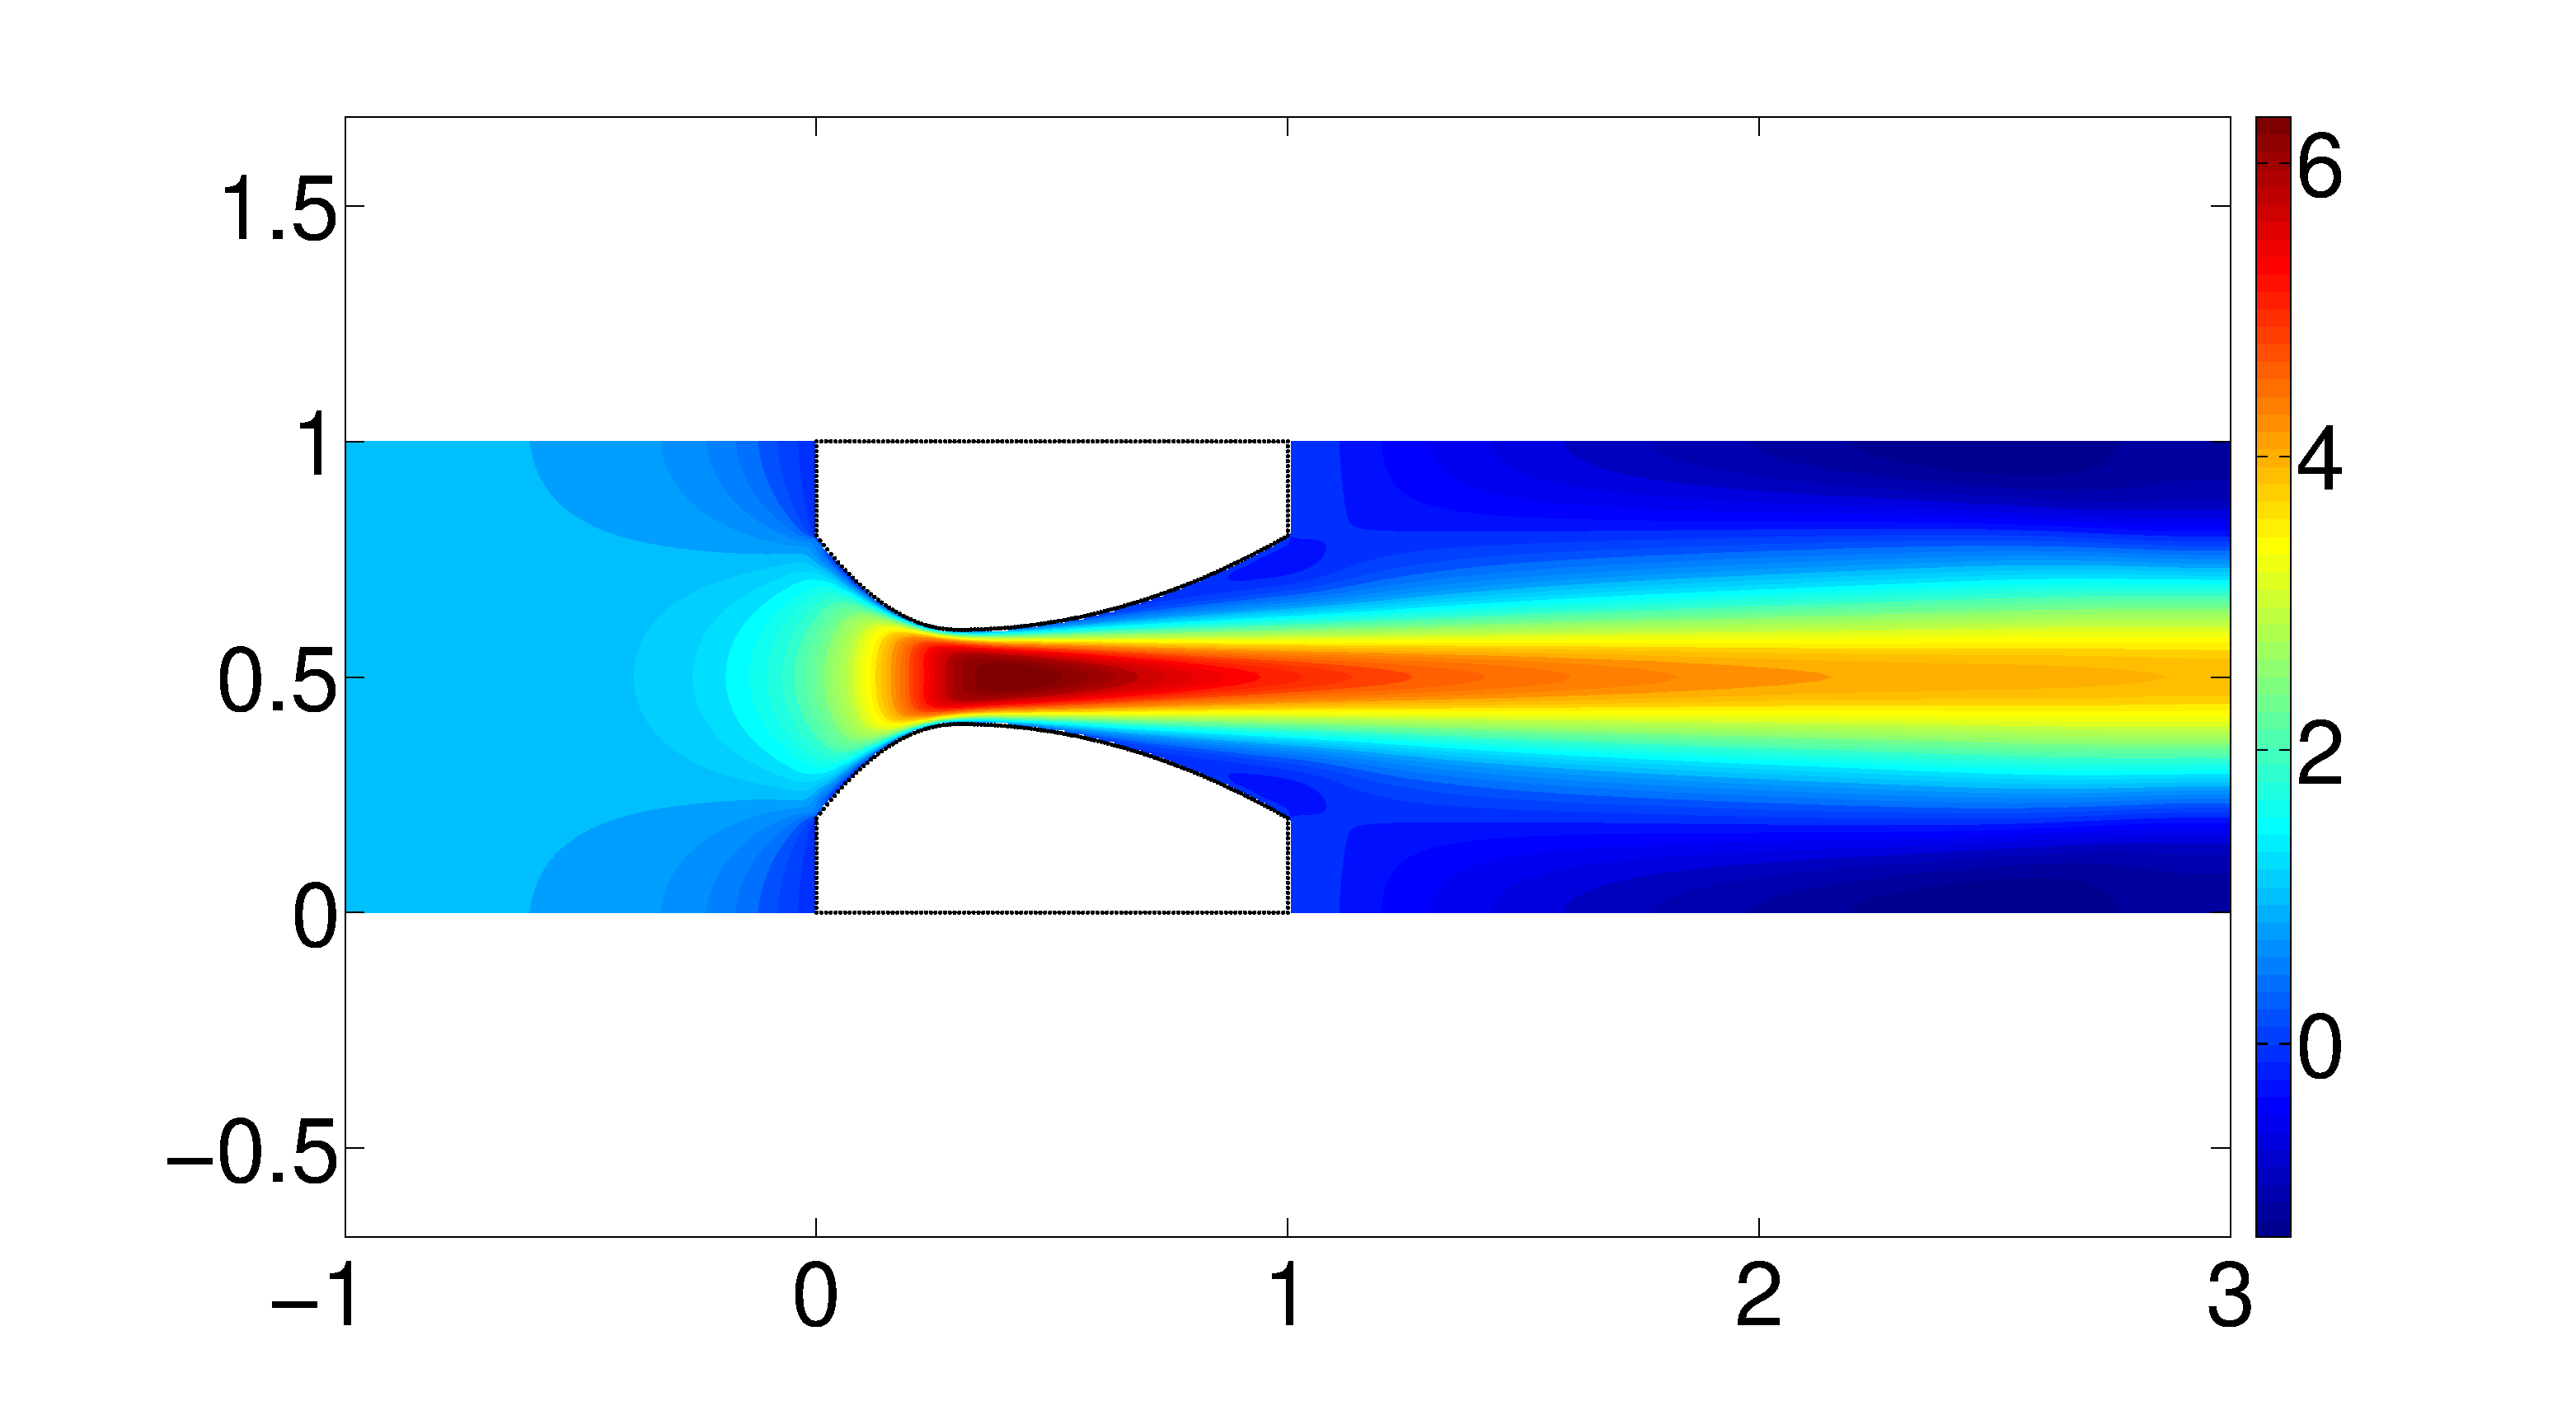
\includegraphics[width=7.0cm]{Chapter_4/figure/flow_through_nozzle/contour_U_RE100.eps}
    }
    \quad
    \subfigure[V-velocity contour.]
    {
    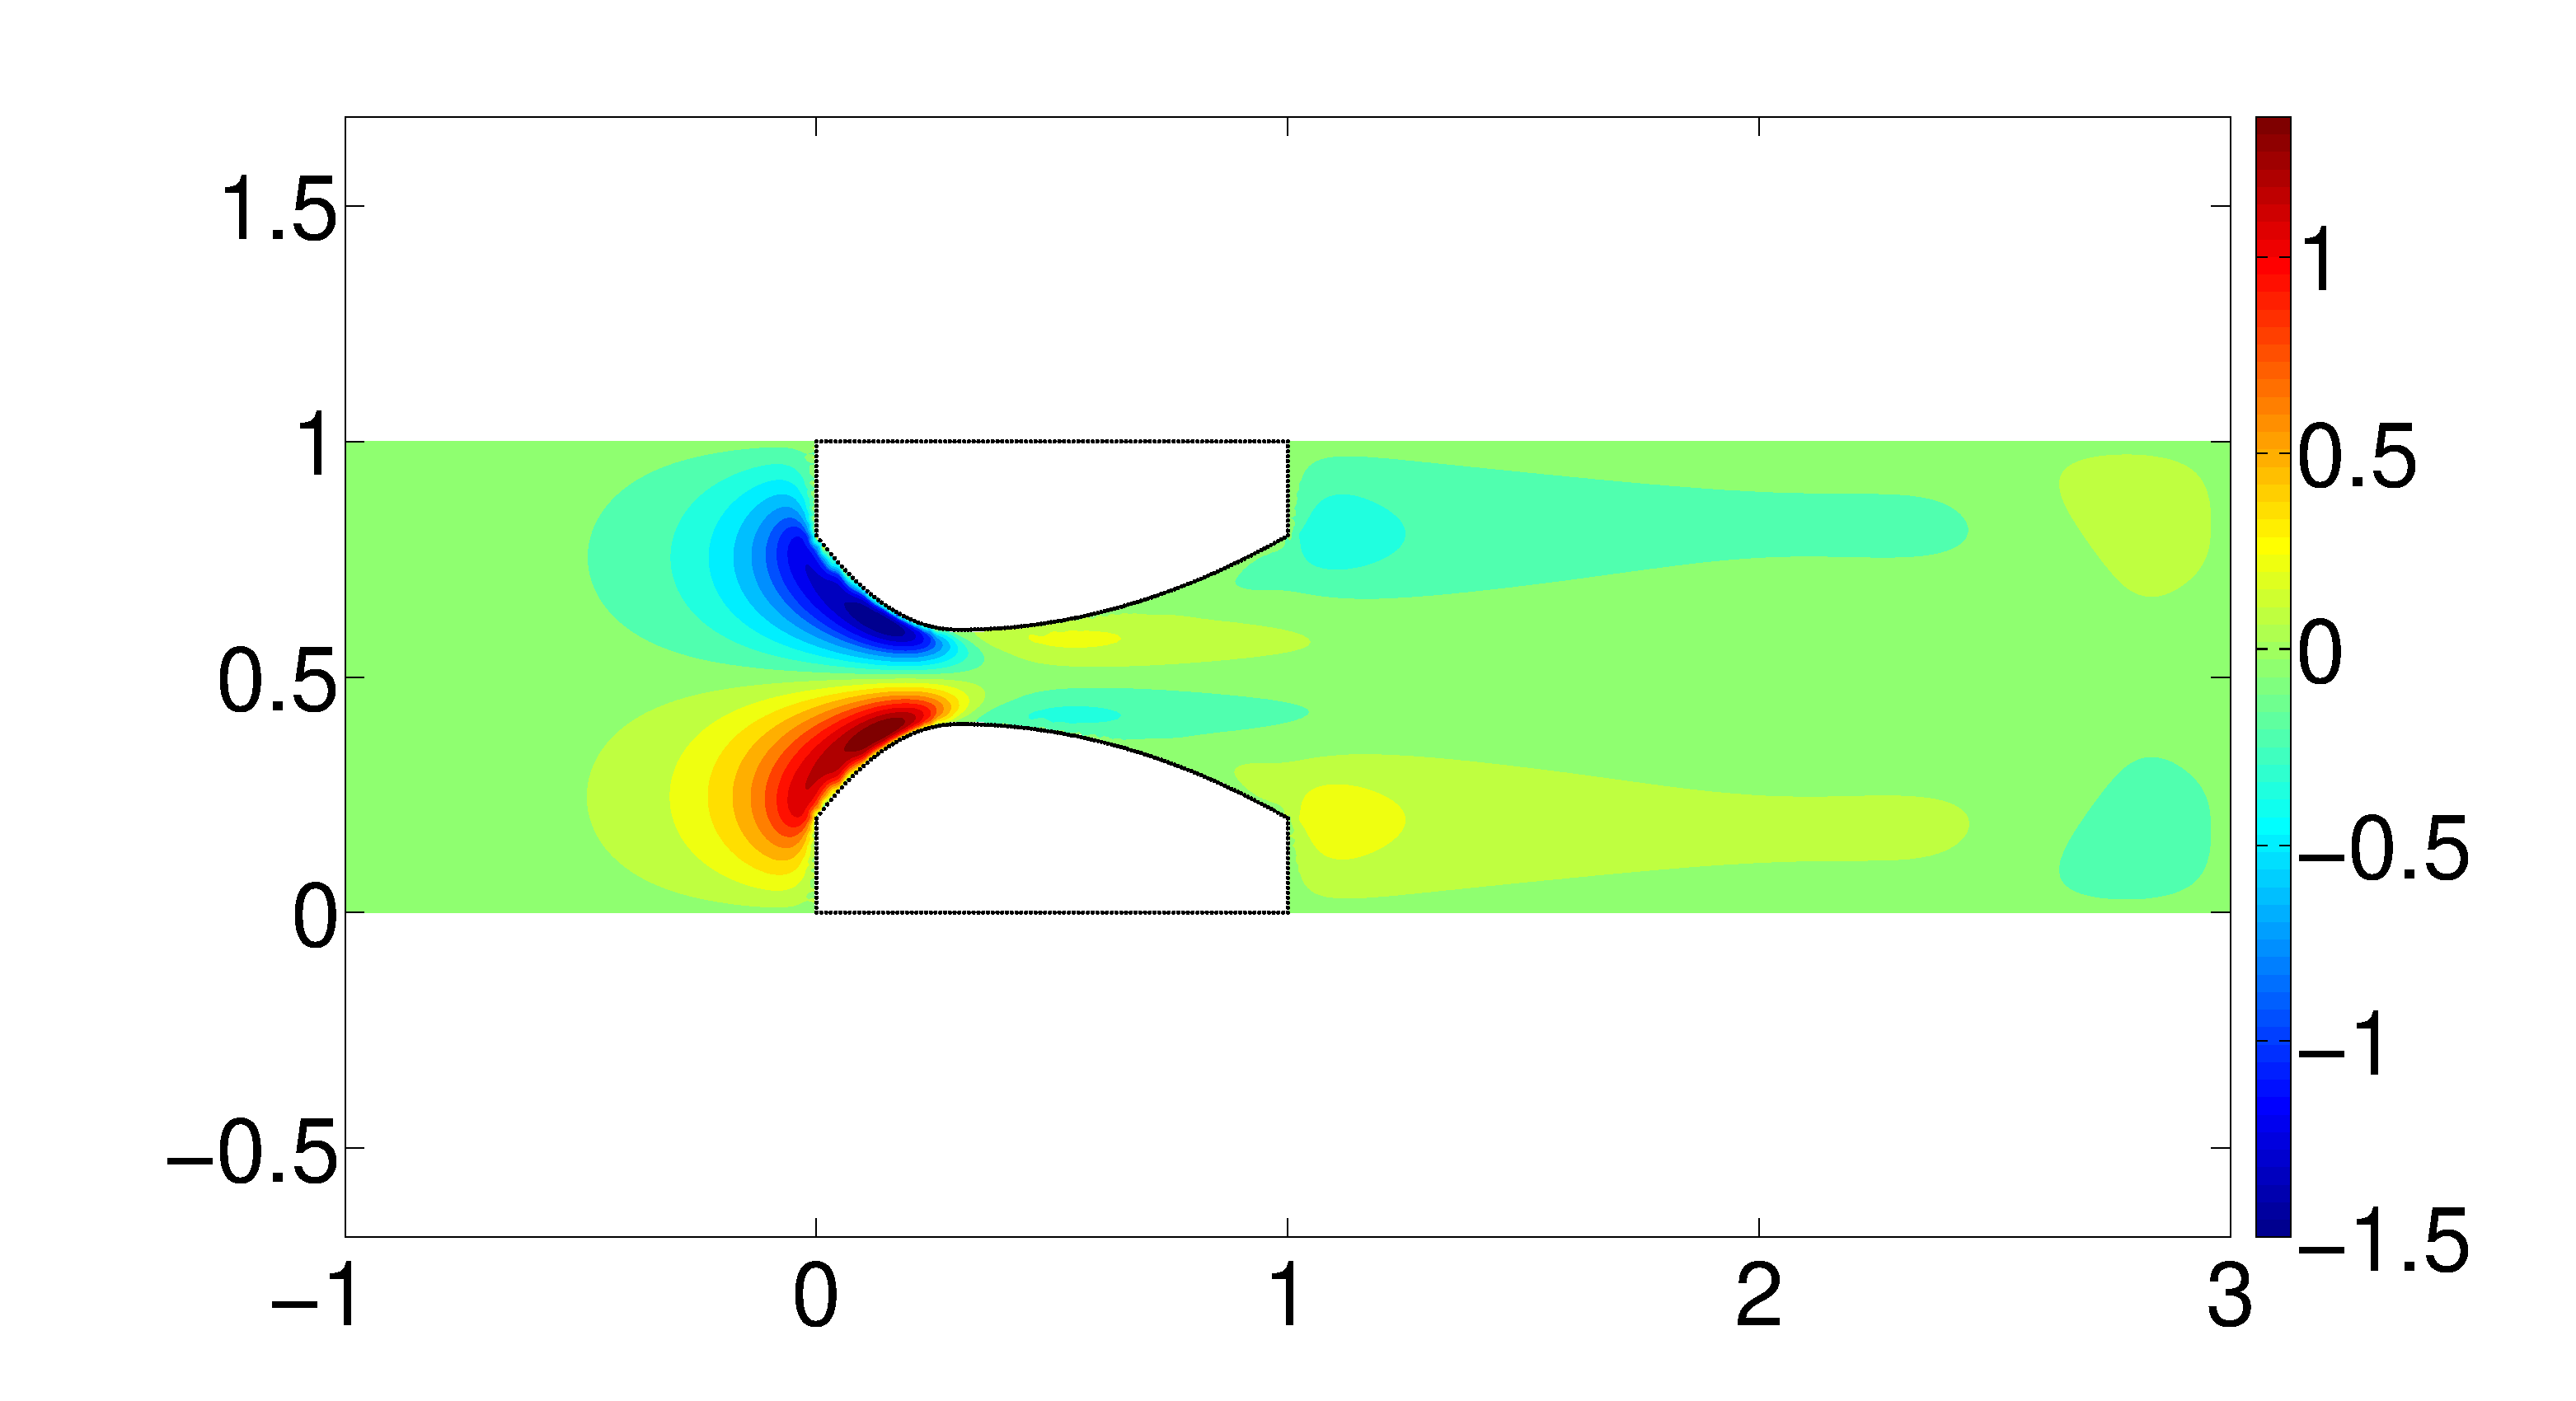
\includegraphics[width=7.0cm]{Chapter_4/figure/flow_through_nozzle/contour_V_RE100.eps}
    }
    \caption{Contour plots for flow through nozzle (Re = 100).}
    \label{fig:C4_nozzleFlow_contourForAnalysis}
\end{figure}

The sensitivity of the flow variables with respect to the throat area is calculated by differentiating the governing equations with respect to the design variable. The boundary conditions do not depend on the shape design variable; therefore, their derivative is equal to zero. This results in zero boundary conditions for the sensitivity equations.

The sensitivity of the flow with respect to the throat area is calculated using CSA. The u-velocity and pressure sensitivities are plotted on the symmetry line of the nozzle; whereas, the v-velocity sensitivity is plotted at the throat area. These values are verified with the complex step results where they showed a favorable comparison. This is shown in Figure \ref{fig:C4_nozzleFlow_sensitivityPlots}.

\begin{figure}[H]
    \centering
    \subfigure[U-velocity sensitivity.]
    {
    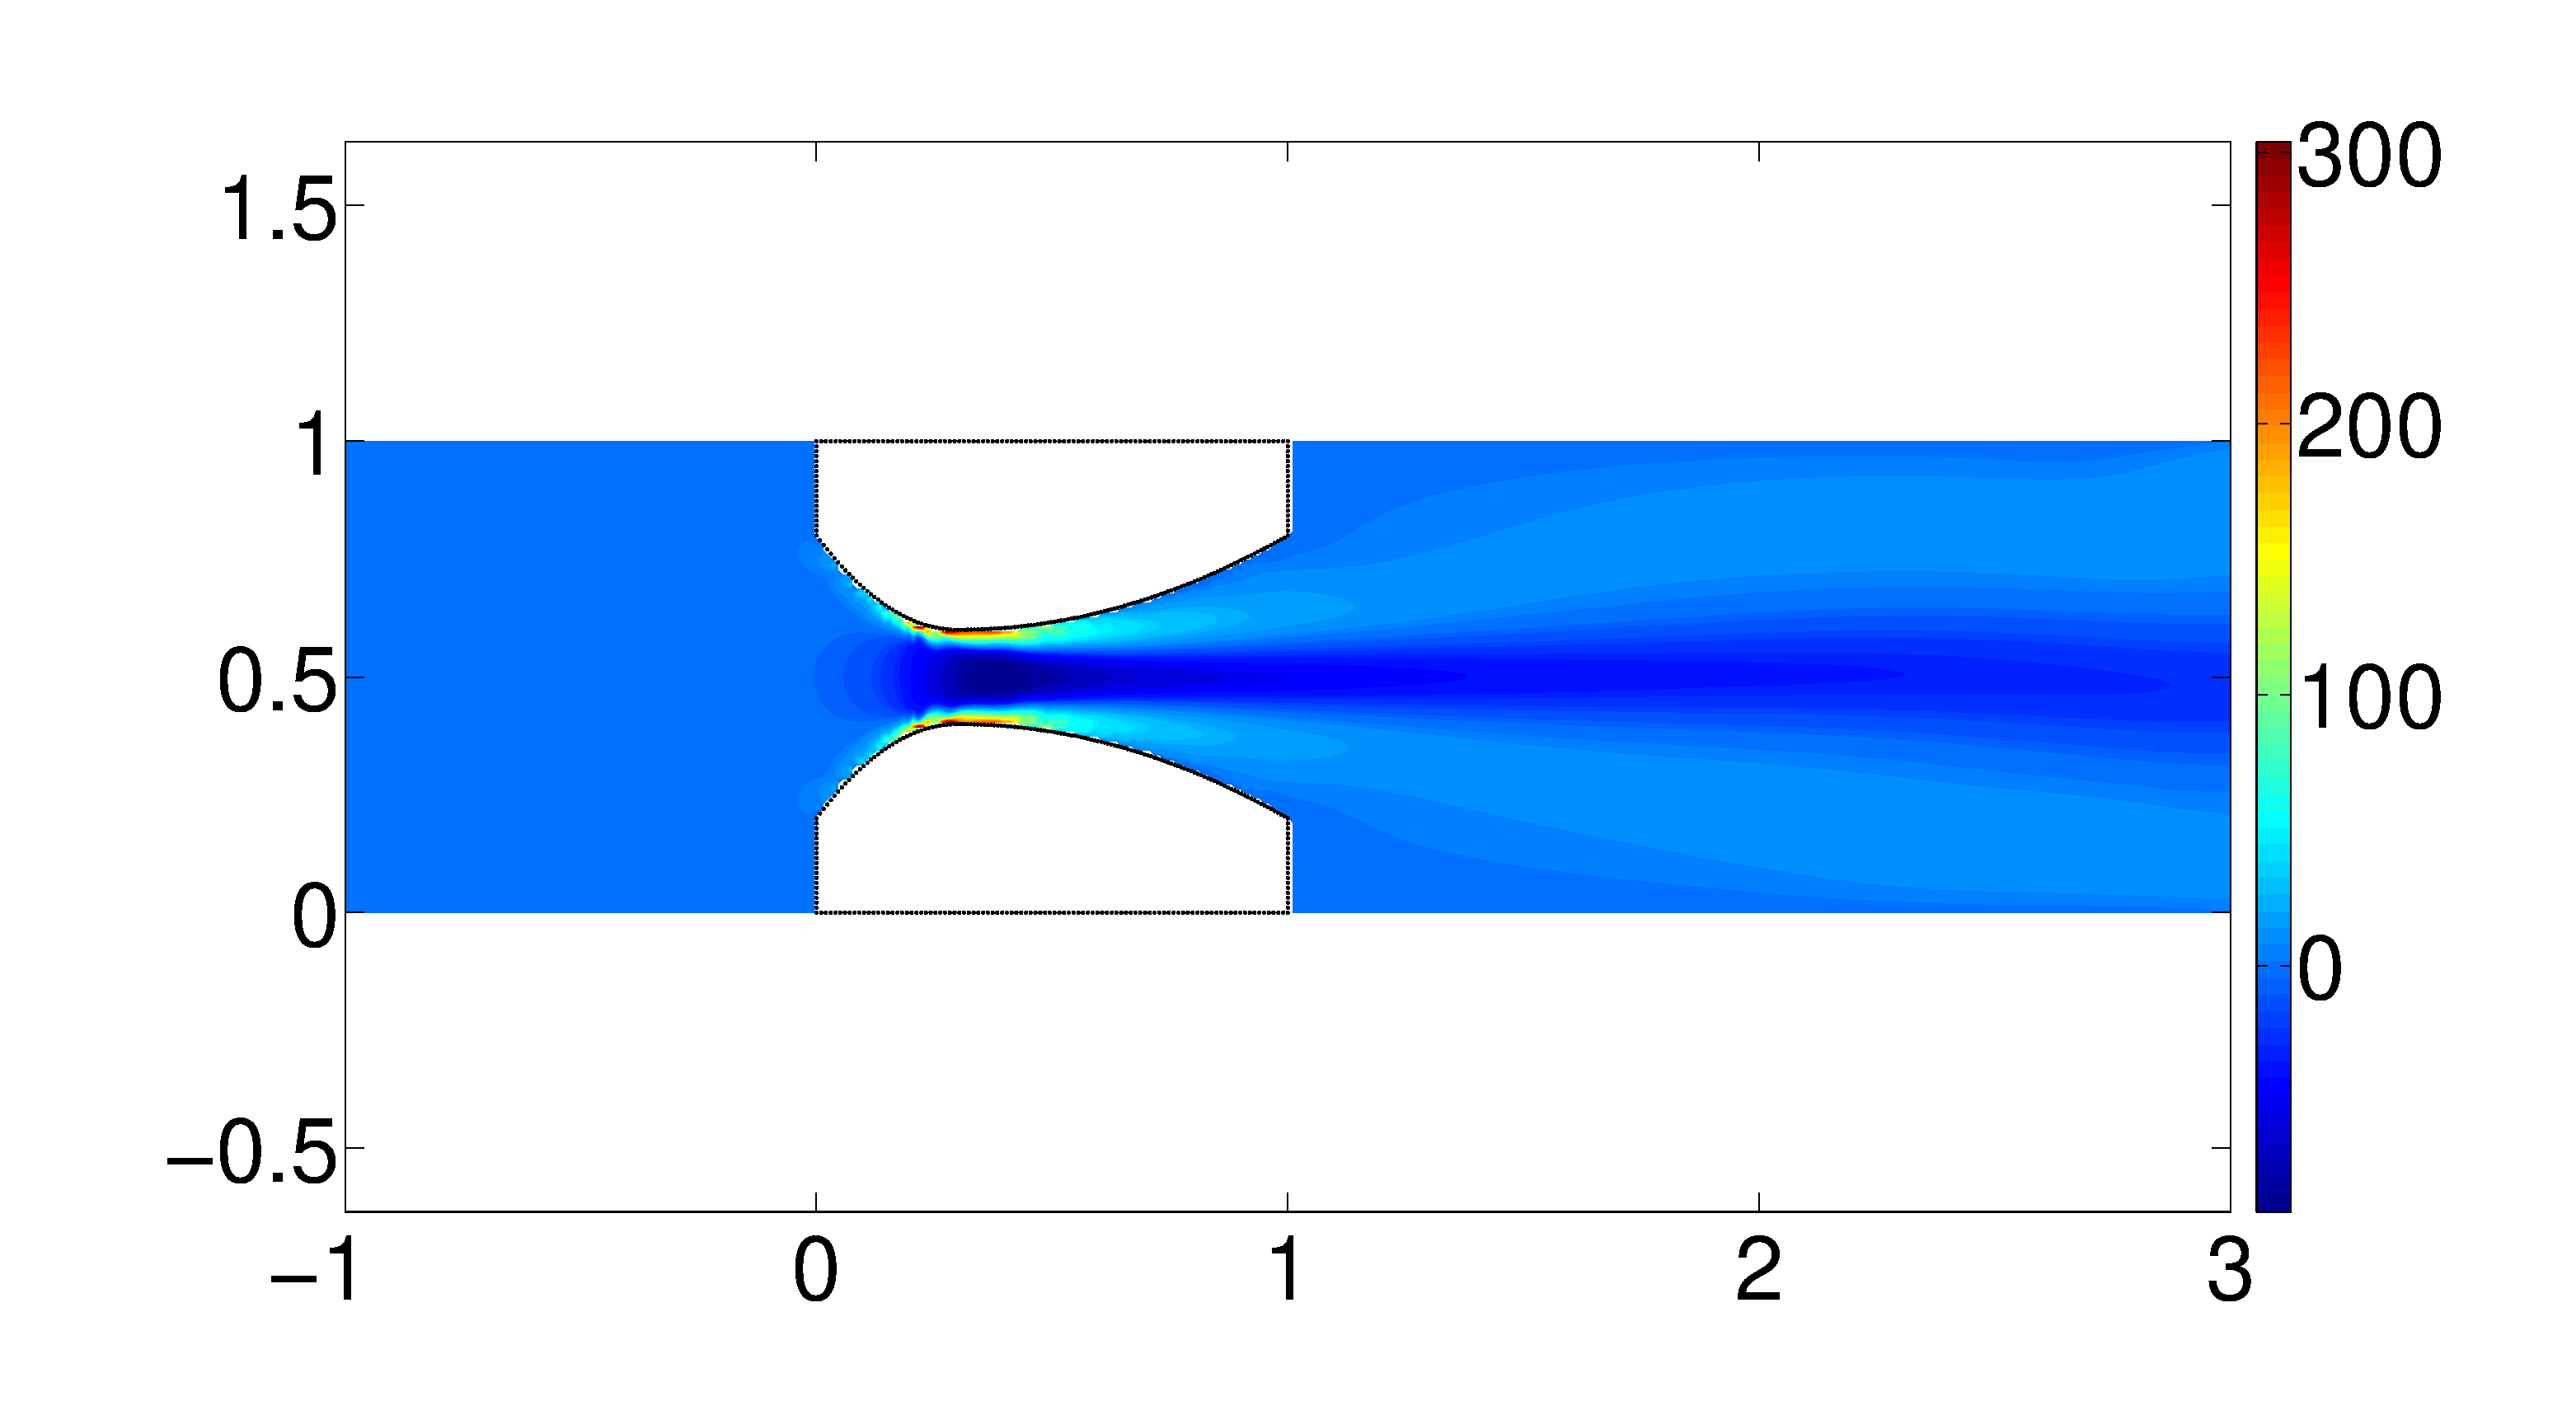
\includegraphics[width=7.0cm]{Chapter_4/figure/flow_through_nozzle/contour_dUdr_RE100.eps}
    }
    \quad
    \subfigure[V-velocity sensitivity.]
    {
    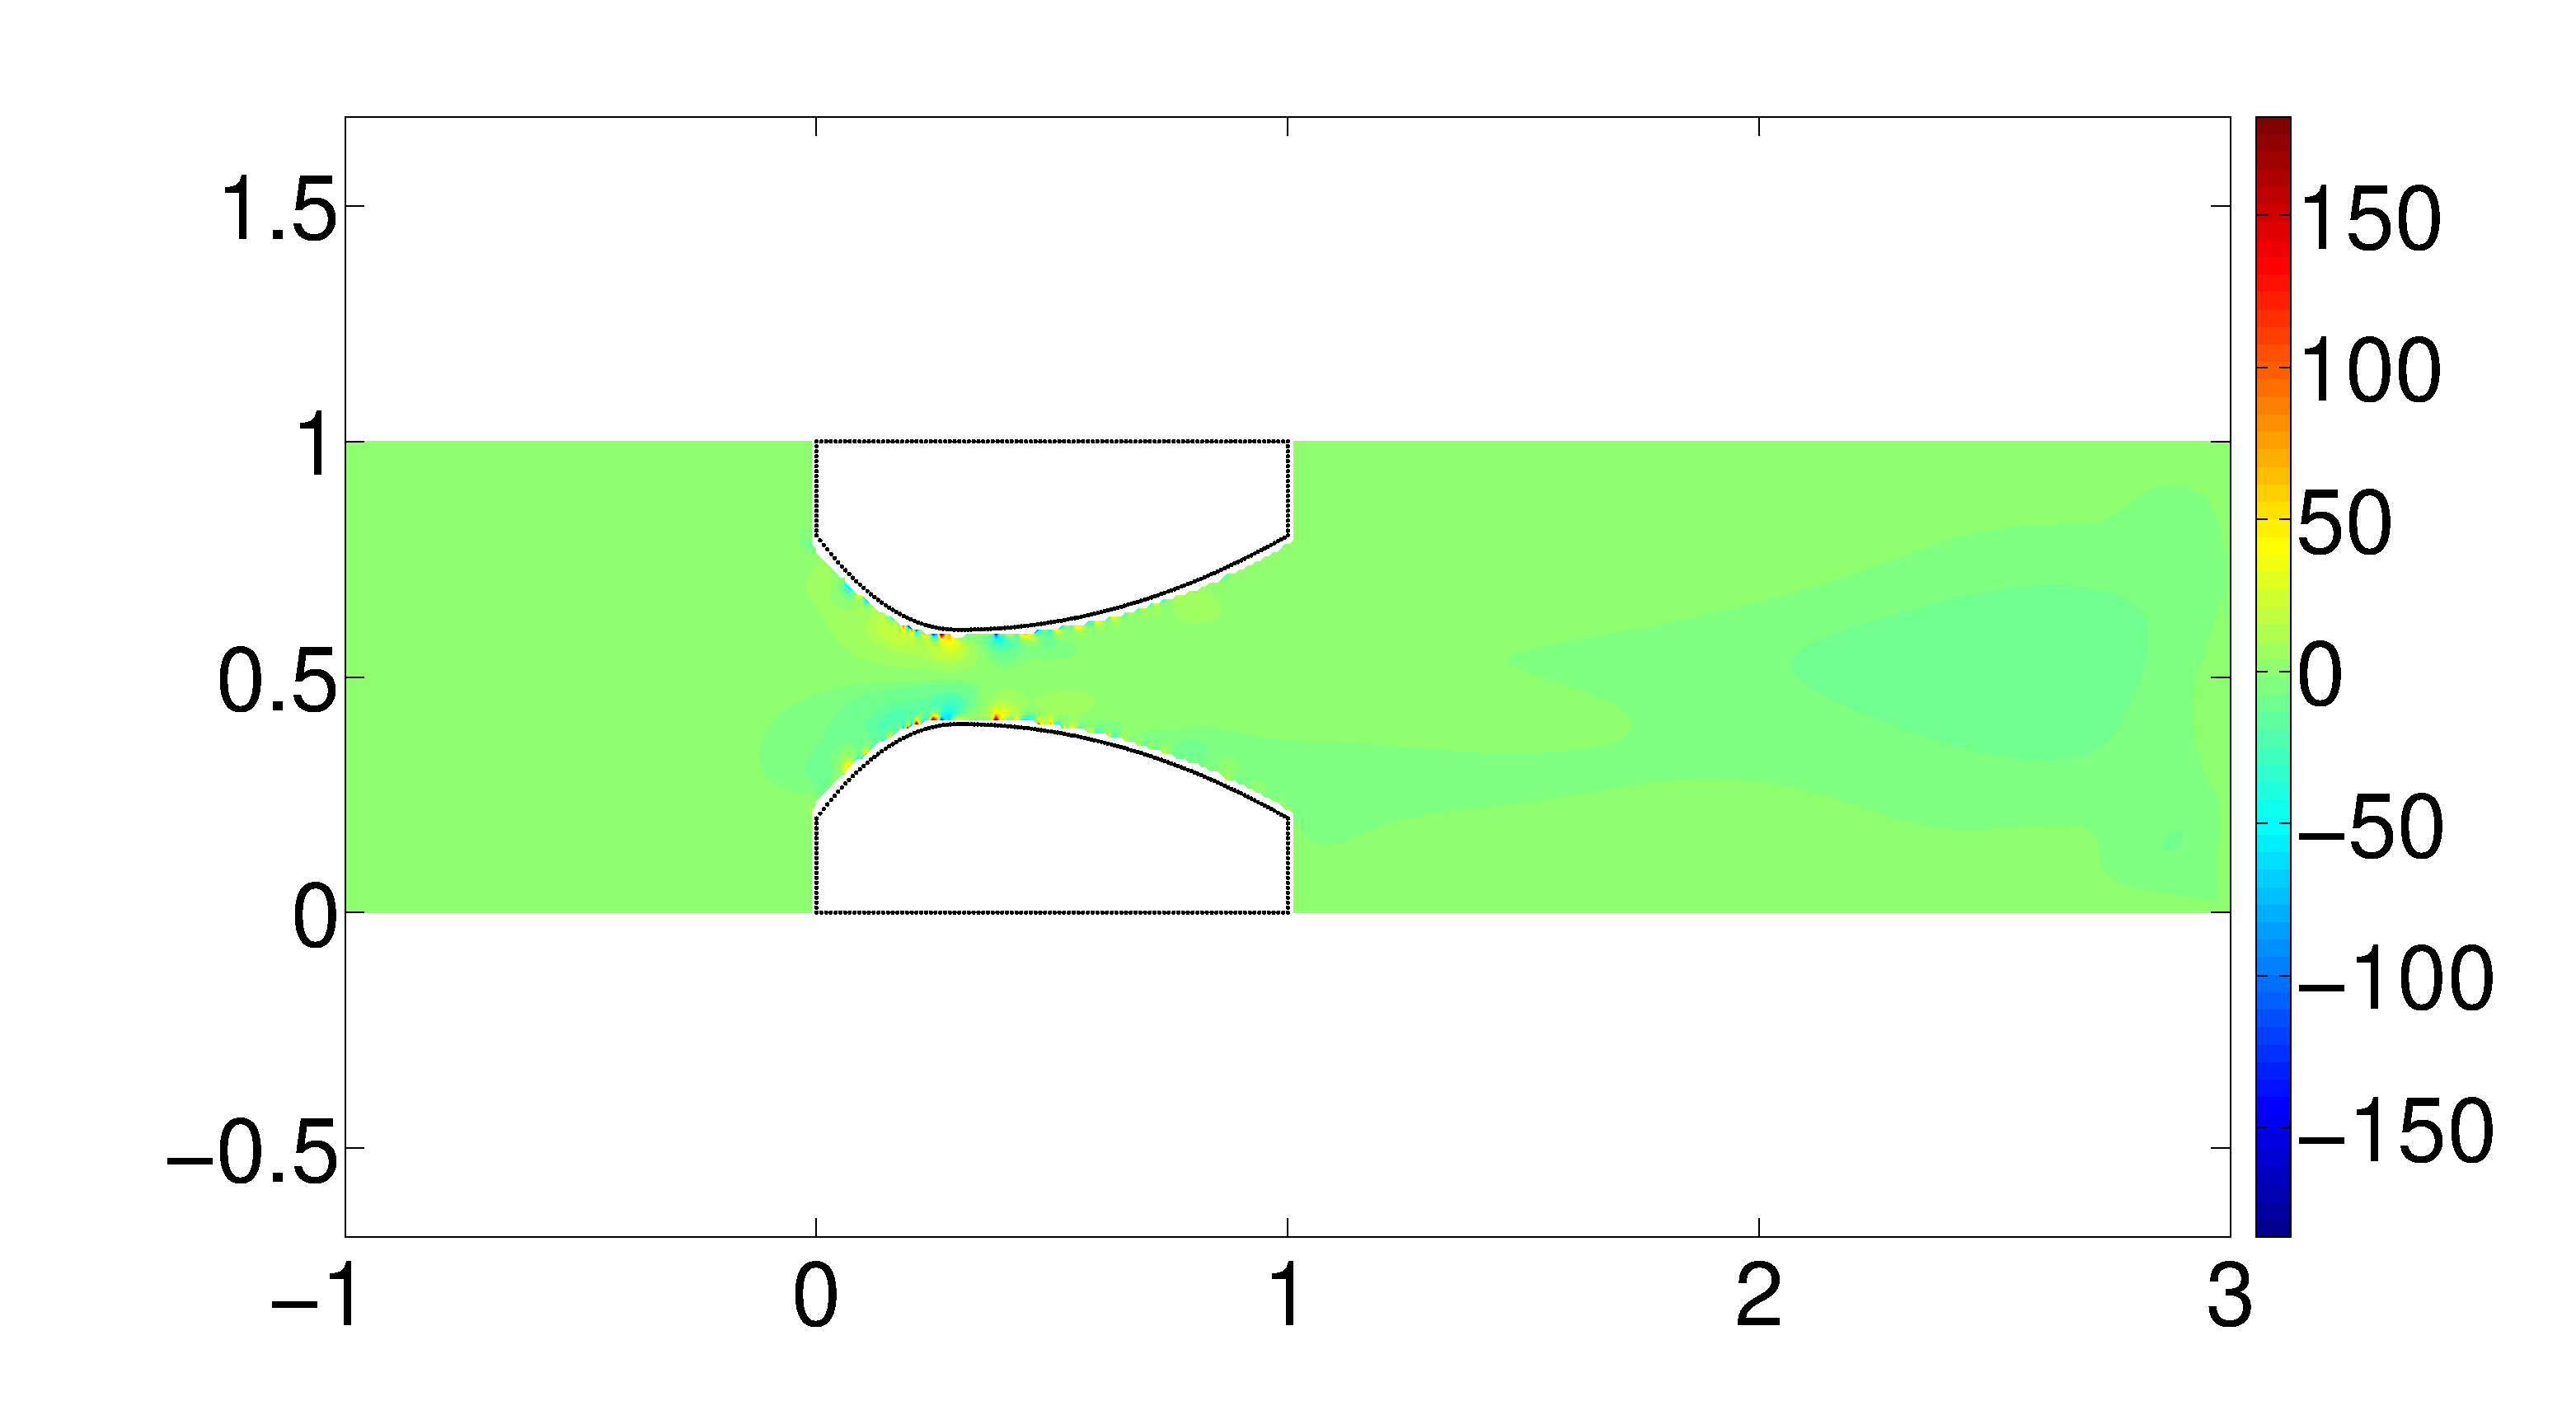
\includegraphics[width=7.0cm]{Chapter_4/figure/flow_through_nozzle/contour_dVdr_RE100.eps}
    }
    \\
    \subfigure[Pressure sensitivity.]
    {
    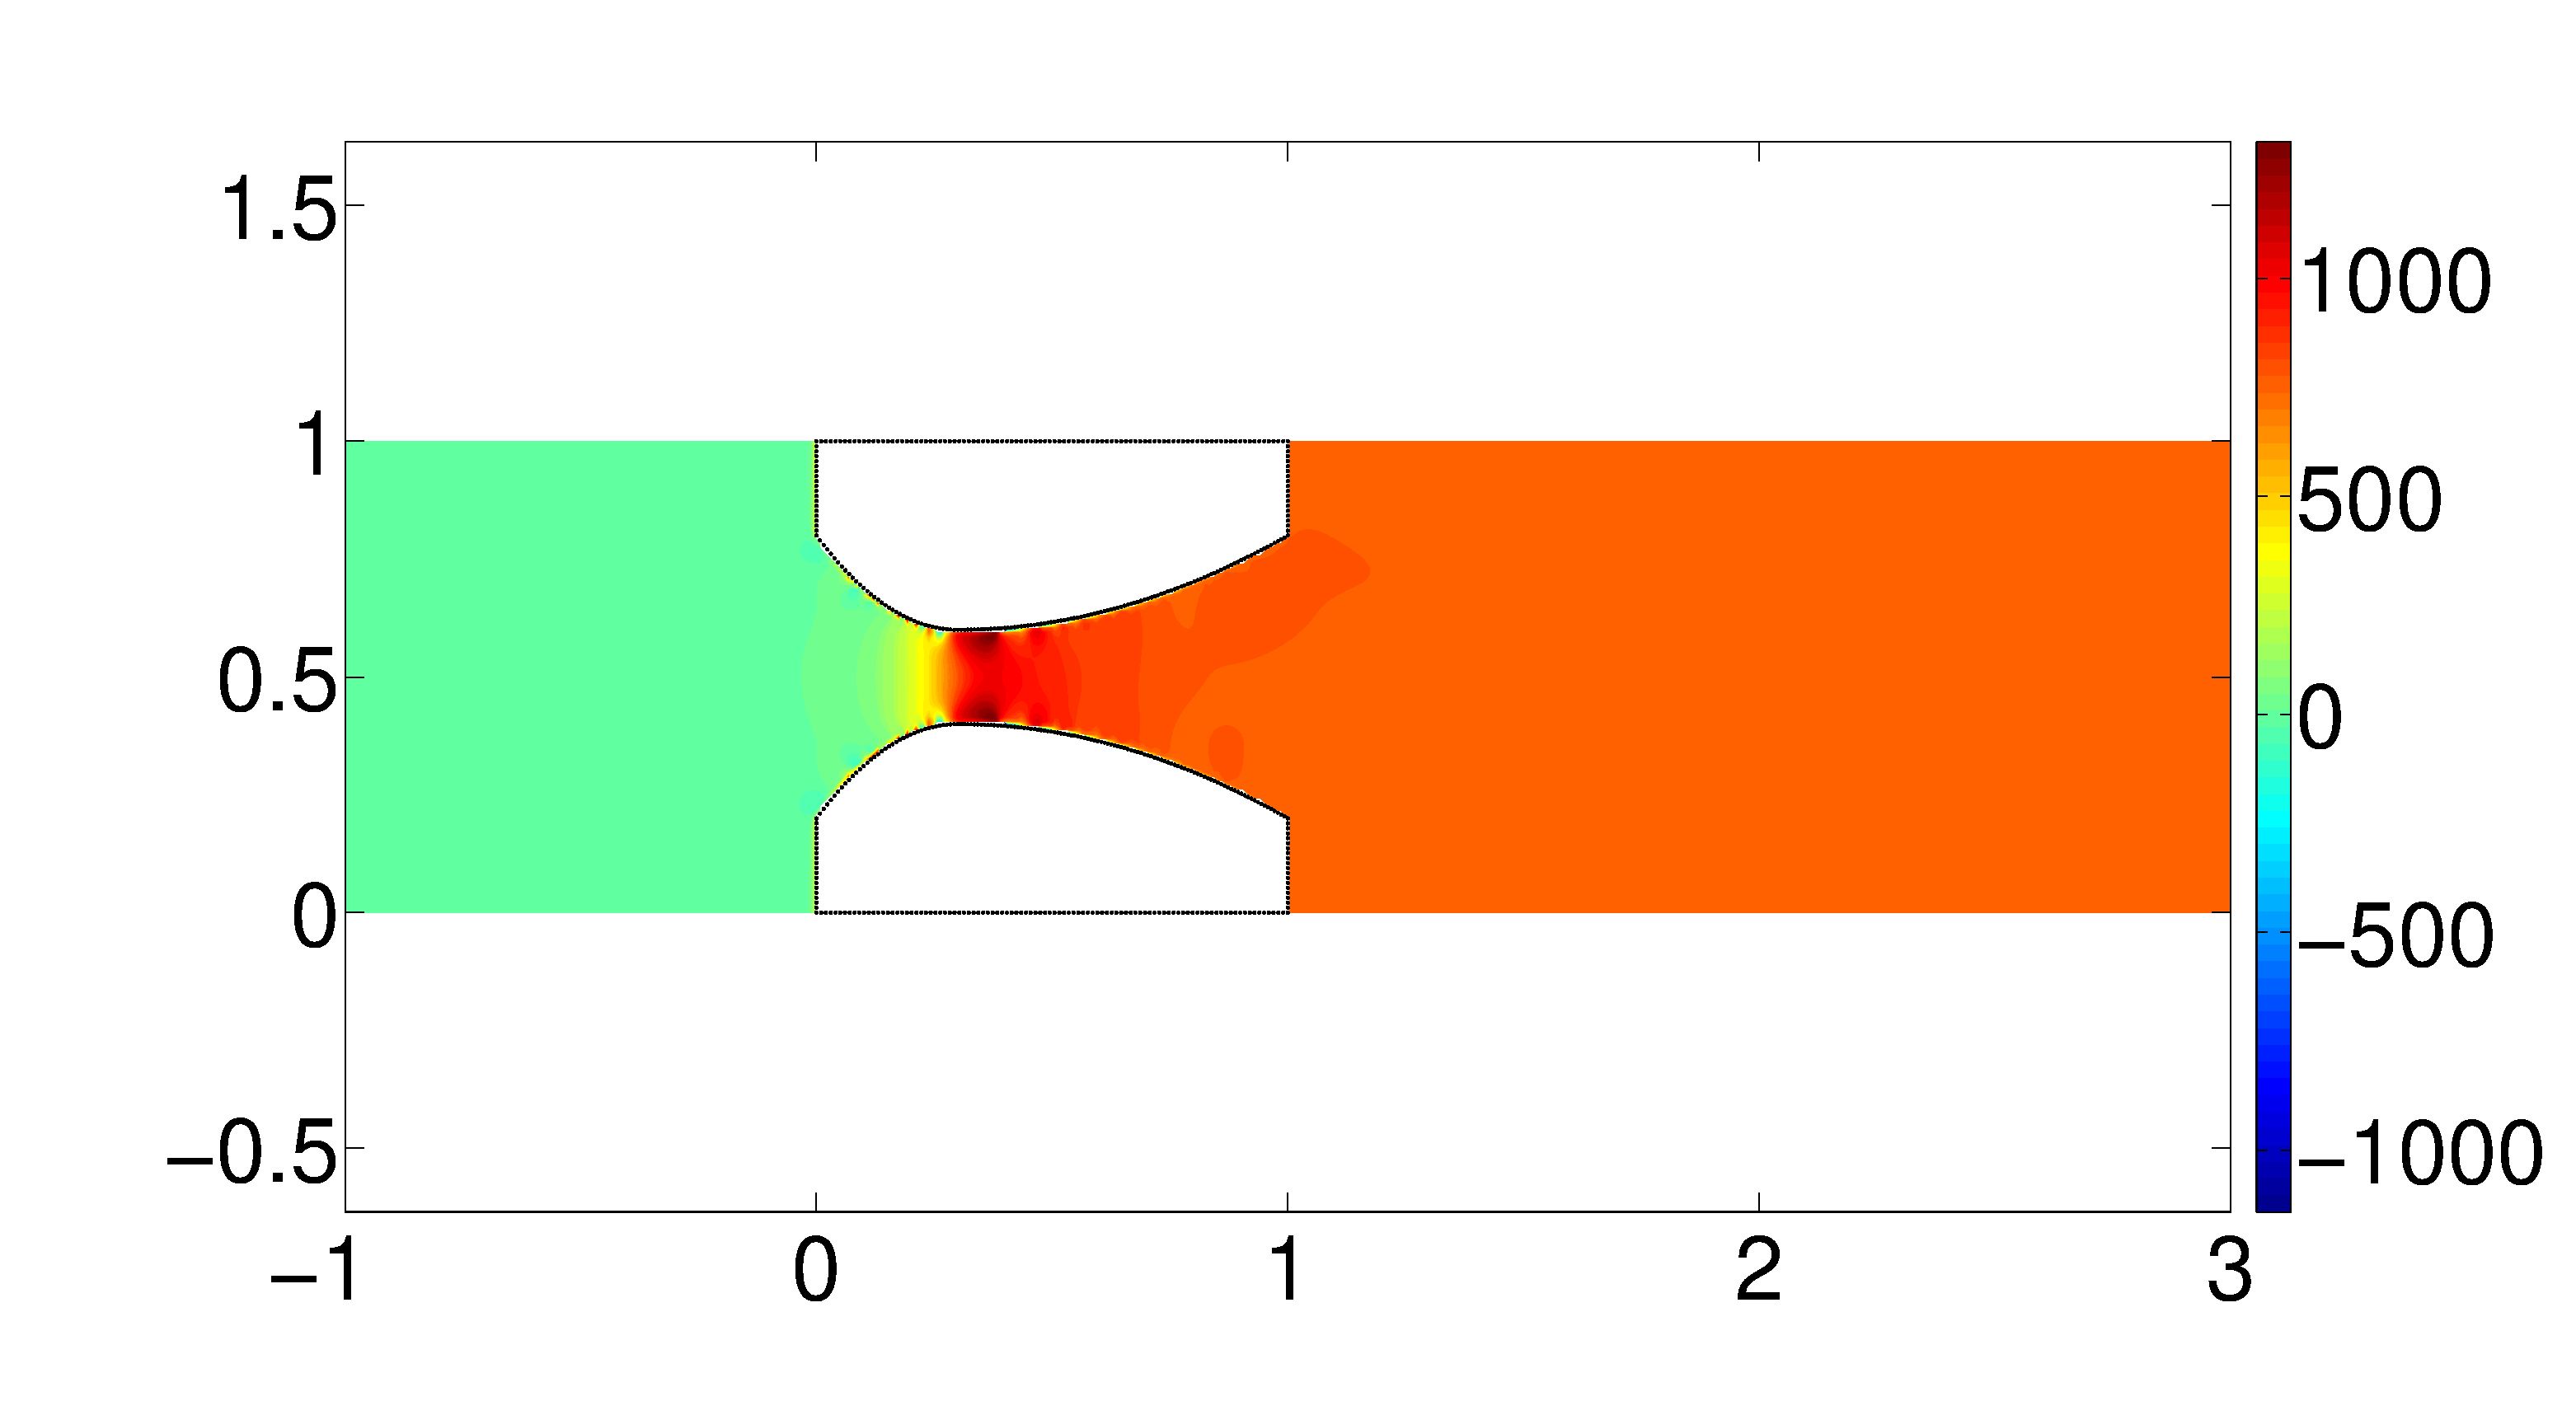
\includegraphics[width=7.0cm]{Chapter_4/figure/flow_through_nozzle/contour_dPdr_RE100.eps}
    }
    \caption{Sensitivity contours.}
    \label{fig:C4_nozzleFlow_sensitivityPlots}
\end{figure}

To verify the sensitivity analysis, the sensitivities of velocity and pressure are plotted on different locations in the domain. We chose the symmetry line of the nozzle to plot the u-velocity and pressure sensitivity with respect to the throat are and the vertical line passing through the throat for verifying the v-velocity sensitivity. The verification is done using the complex step sensitivities as shown in Figure \ref{fig:C4_nozzleSensitivityVerification}.

\begin{figure}[H]
    \centering
    \subfigure[U-velocity sensitivity on $y = 0.5$.]
    {
    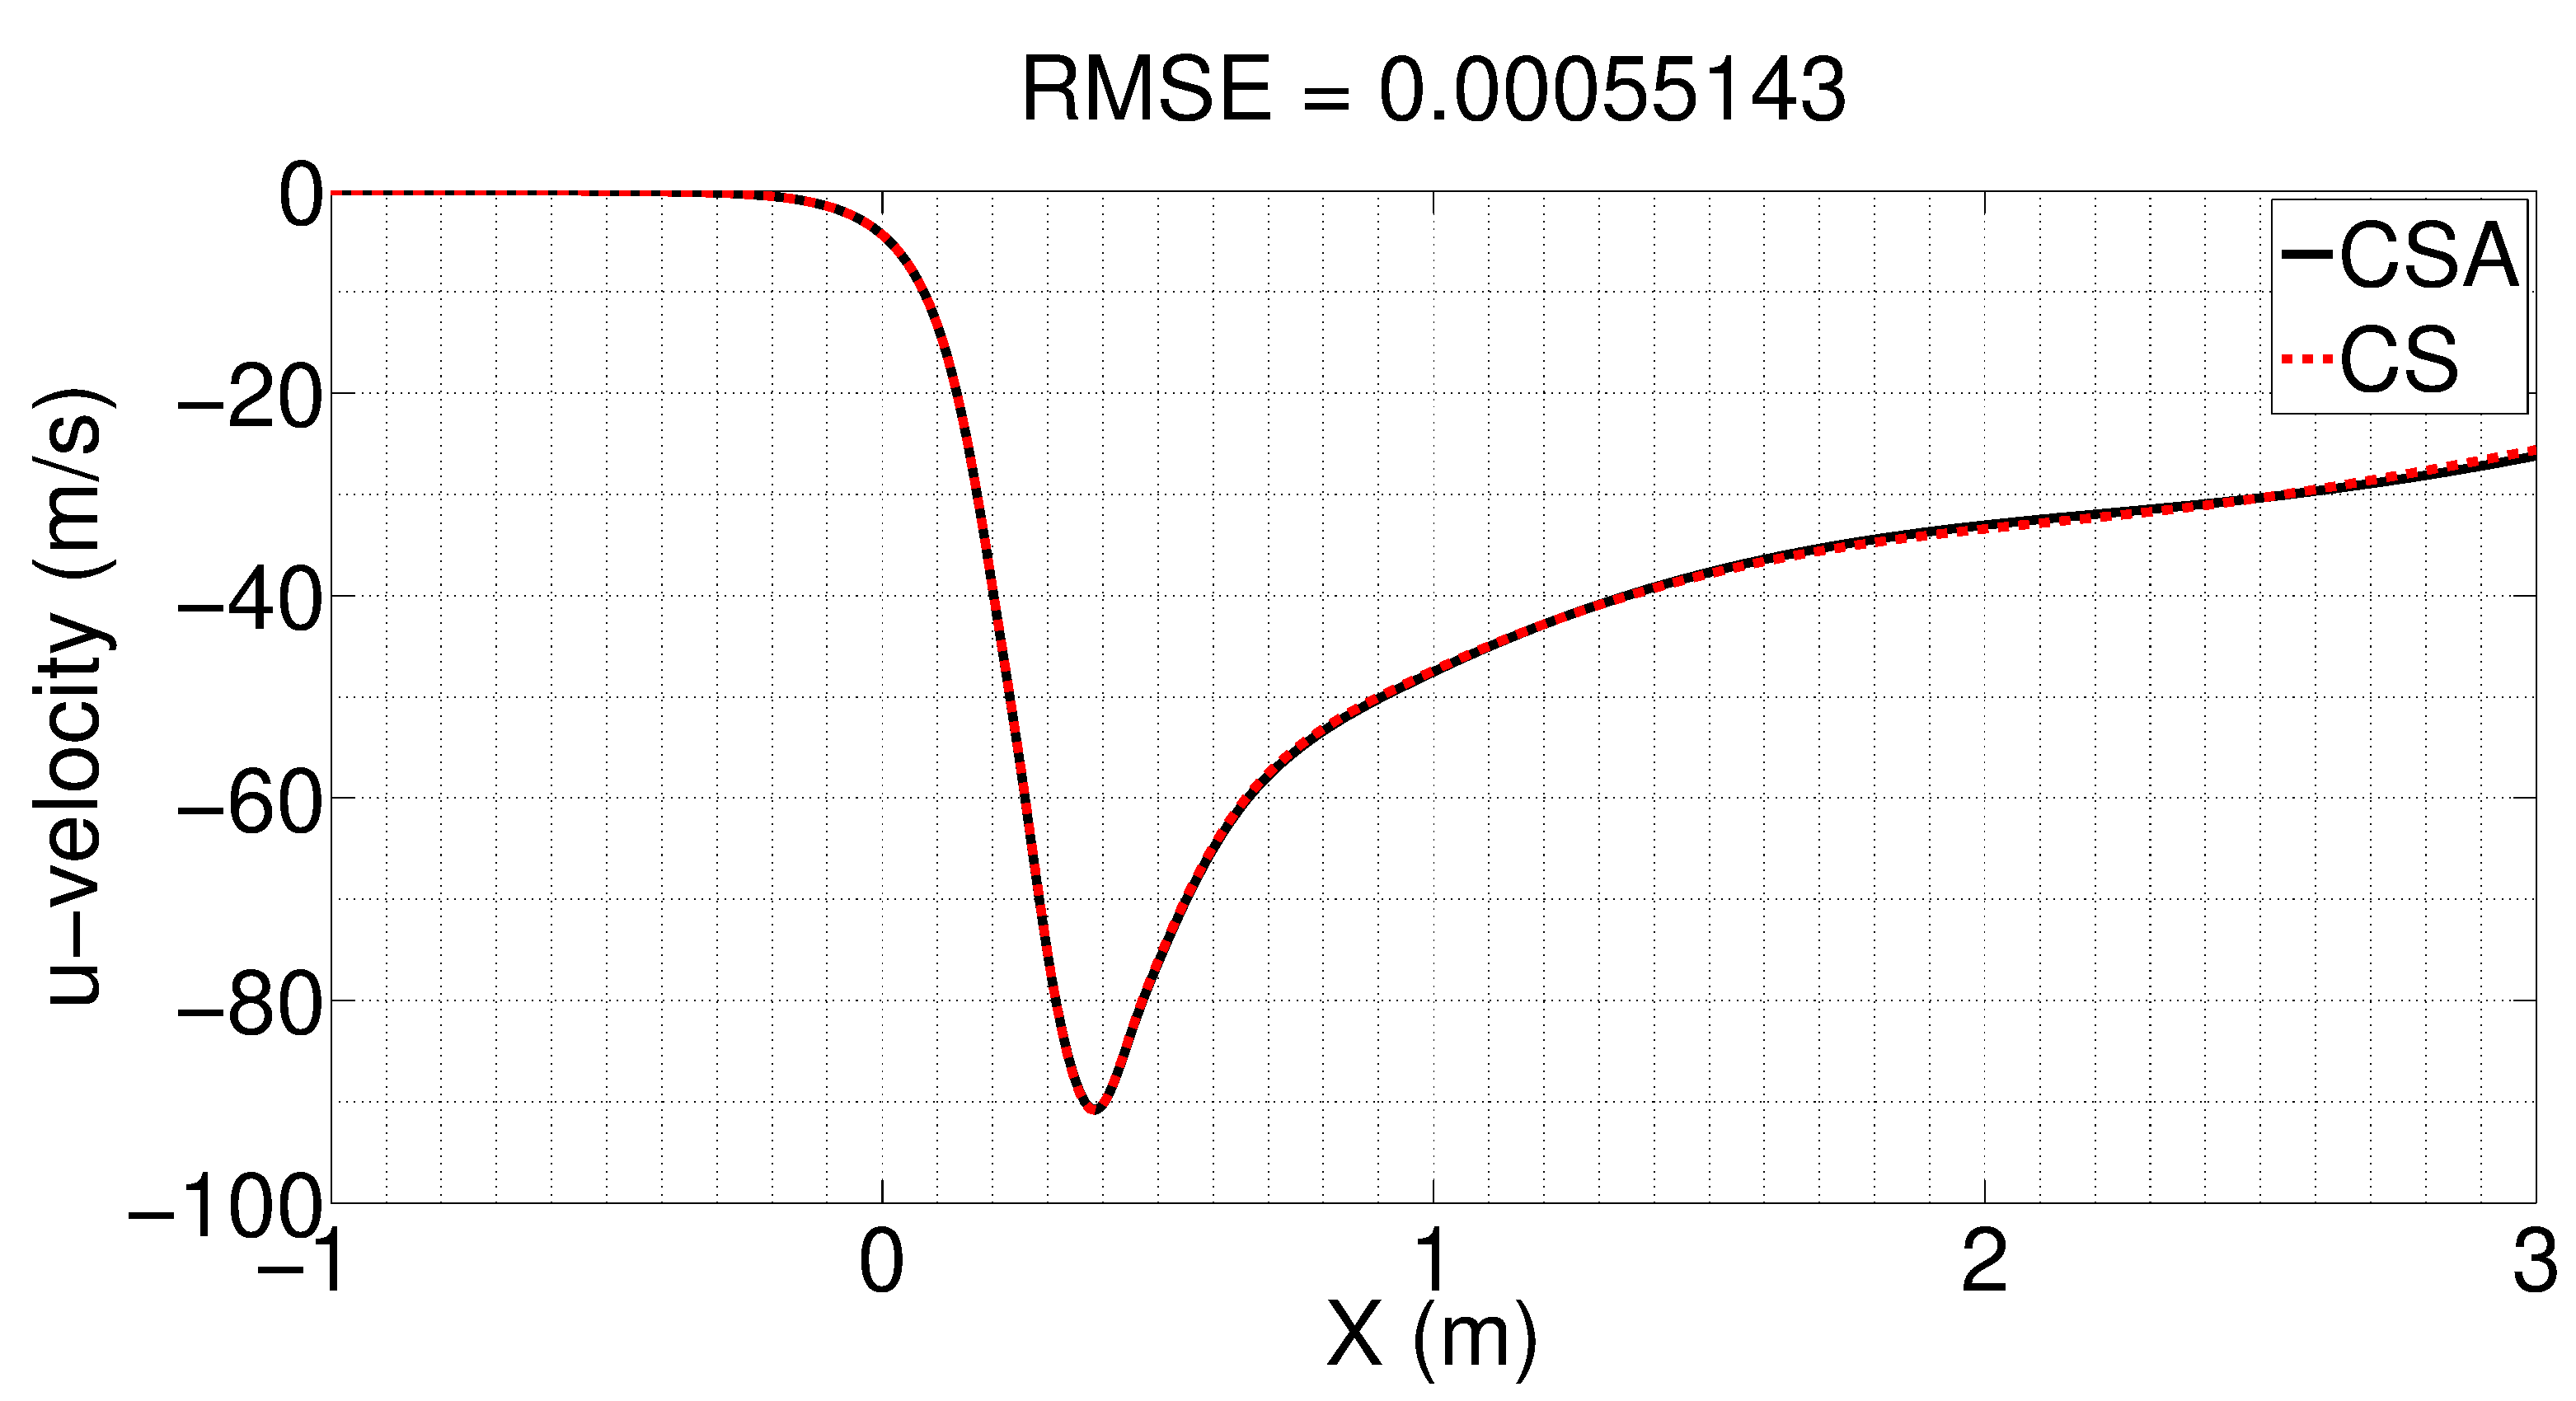
\includegraphics[width=7.0cm]{Chapter_4/figure/flow_through_nozzle/verification_dUdr_RE100_Y050.eps}
    }
    \quad
    \subfigure[V-velocity sensitivity on $x = 0.3$.]
    {
    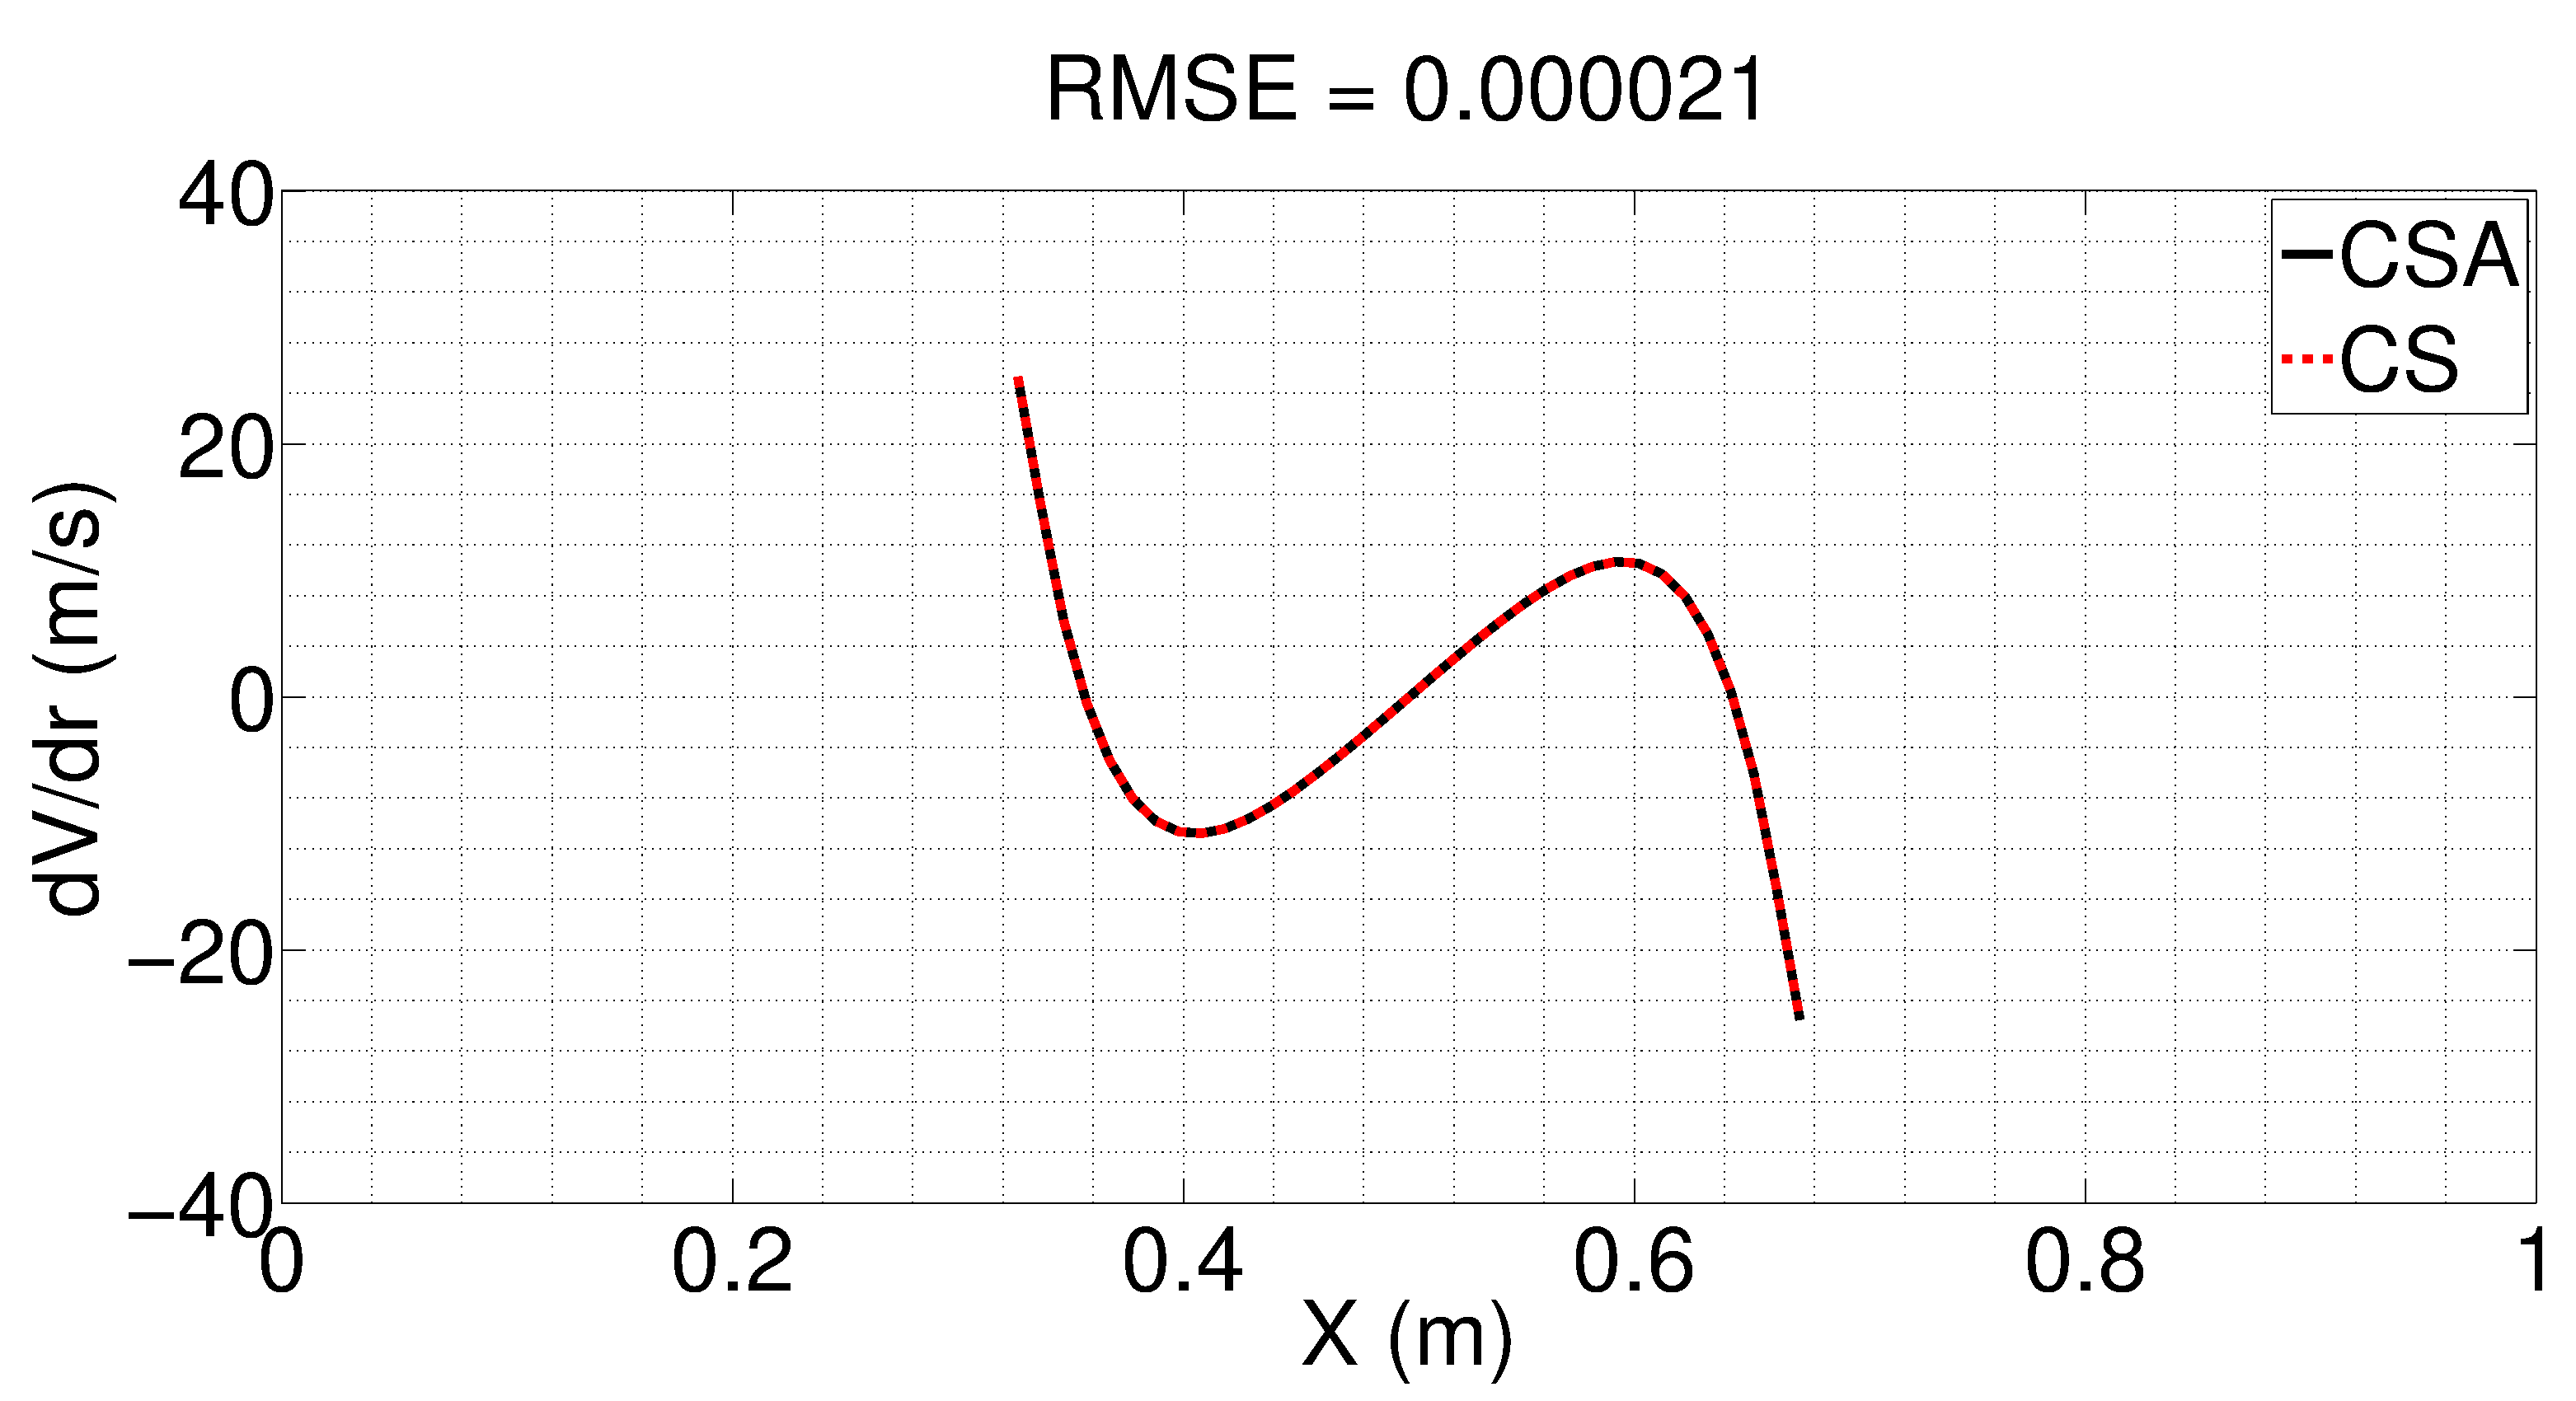
\includegraphics[width=7.0cm]{Chapter_4/figure/flow_through_nozzle/verification_dVdr_RE100_X030.eps}
    }
    \\
    \subfigure[Pressure sensitivity on $y = 0.5$.]
    {
    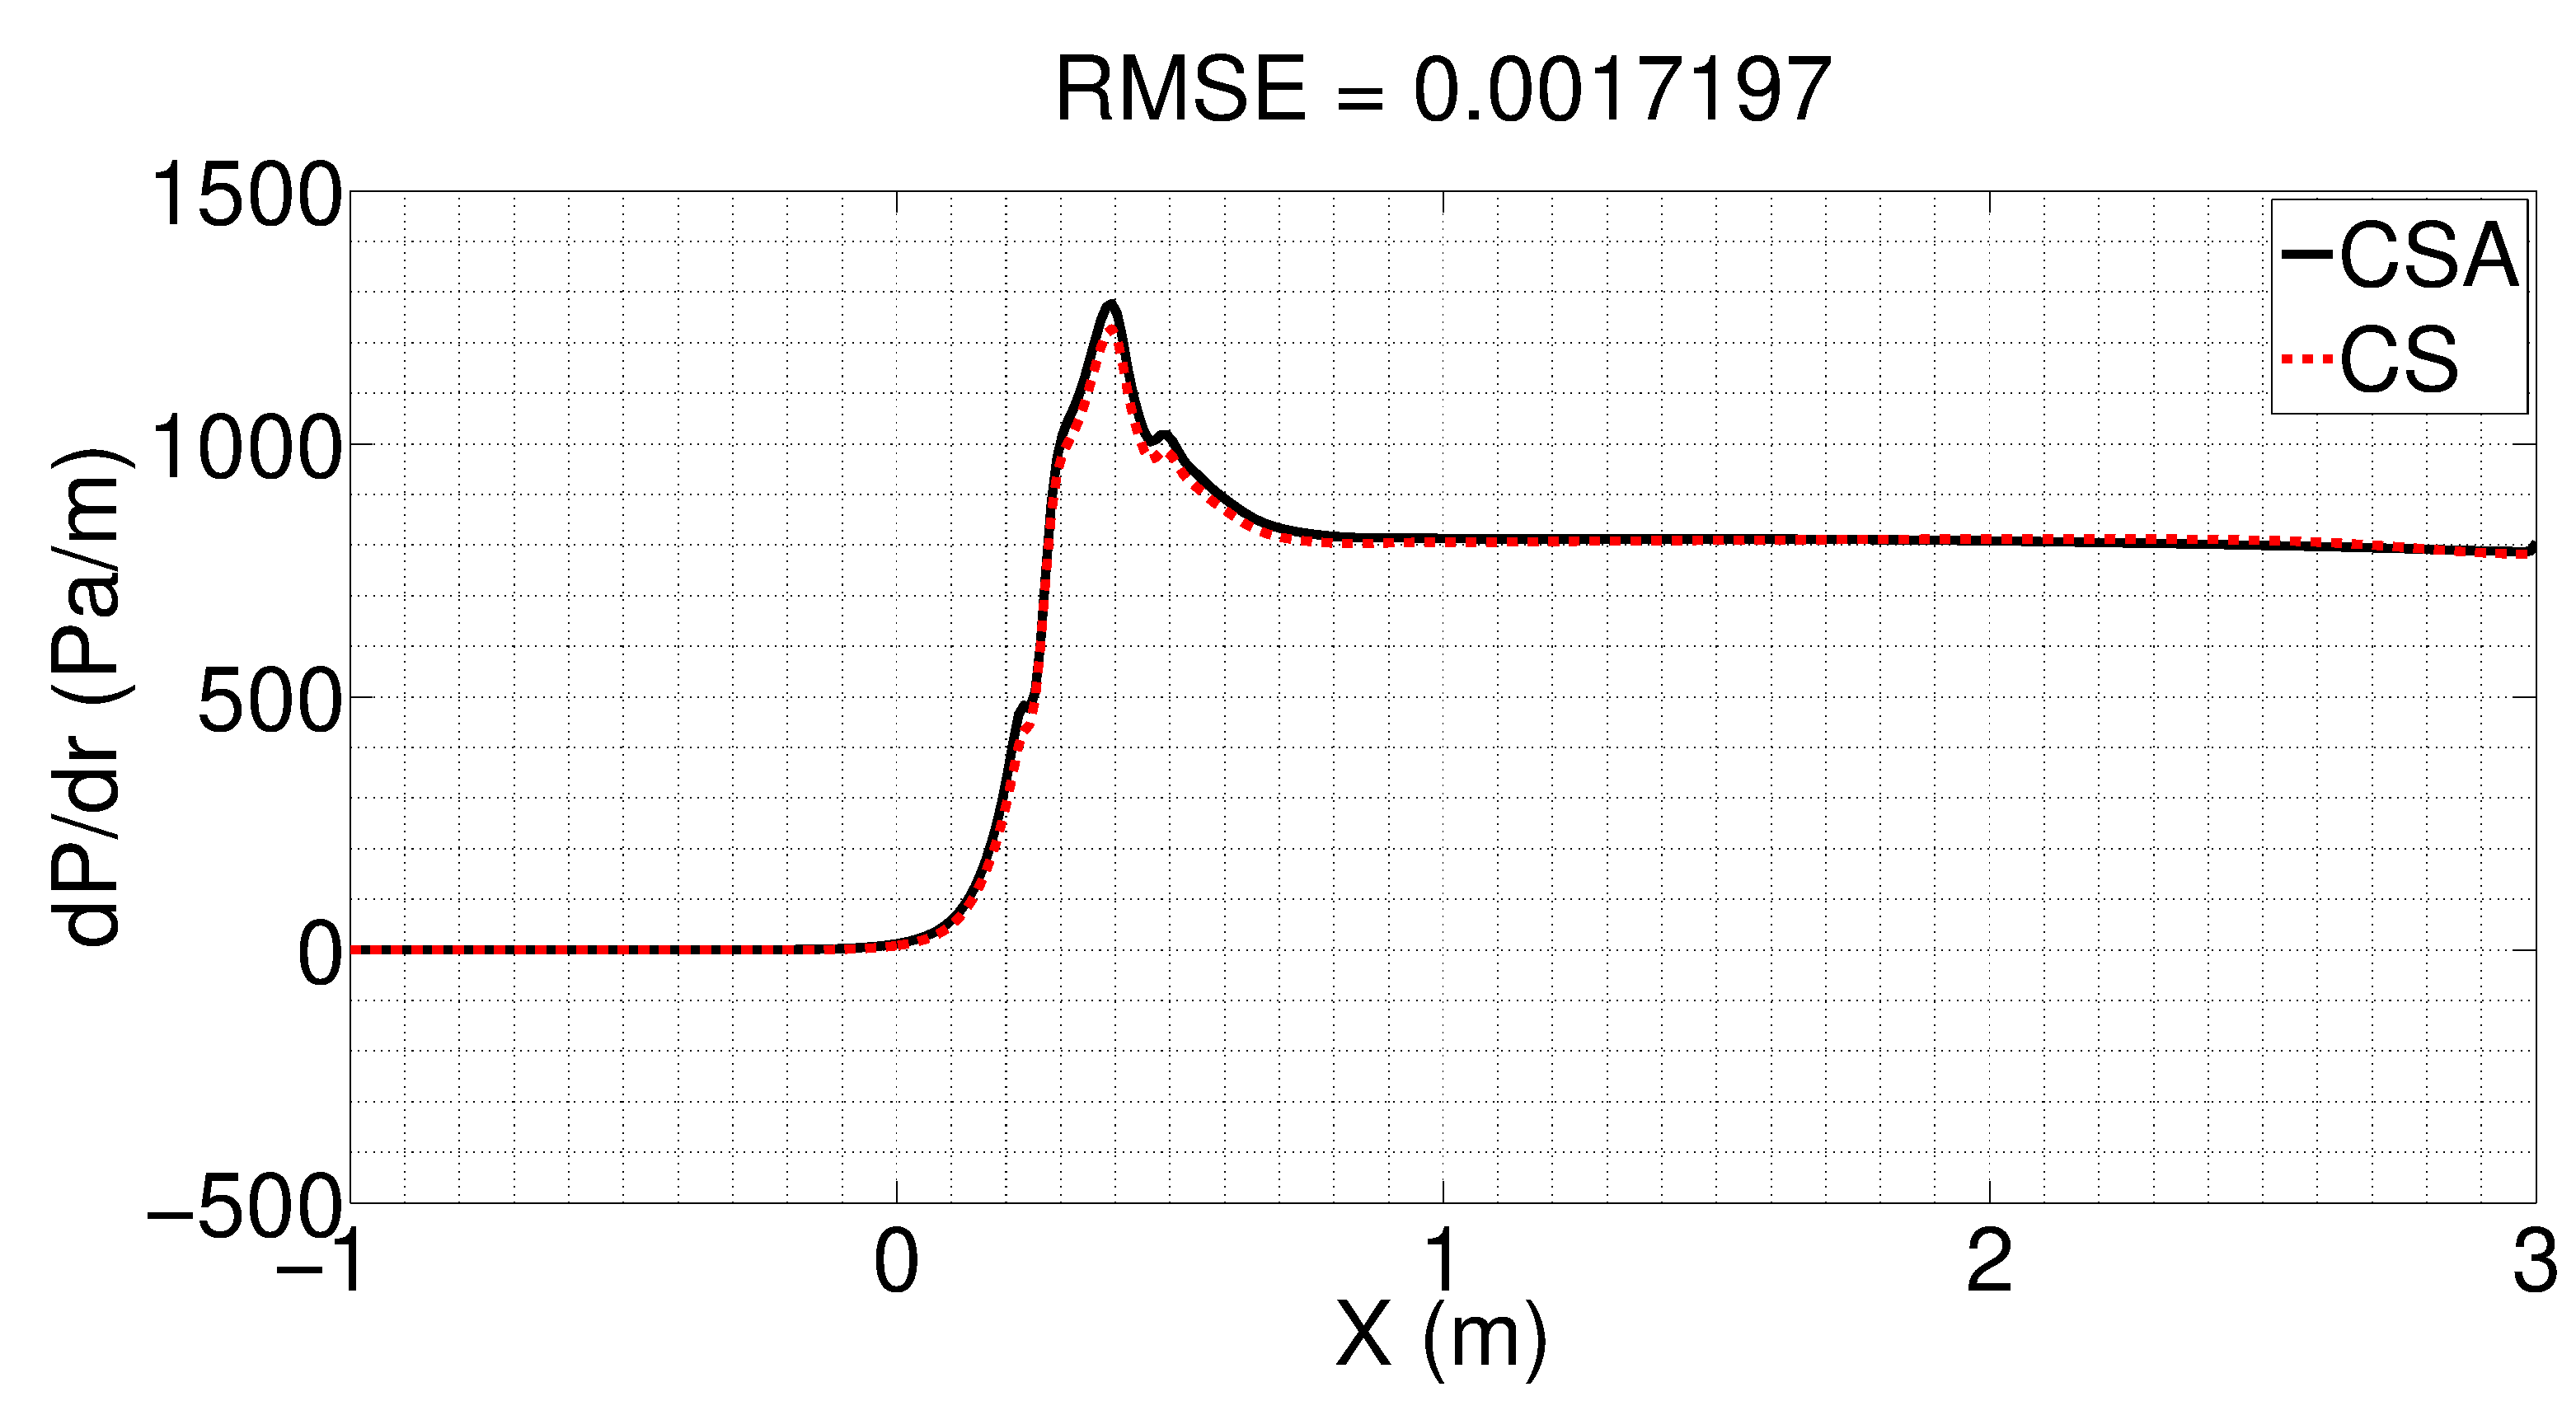
\includegraphics[width=7.0cm]{Chapter_4/figure/flow_through_nozzle/verification_dPdr_RE100_Y050.eps}
    }
    \caption{Verification of sensitivity results for the nozzle.}
    \label{fig:C4_nozzleSensitivityVerification}
\end{figure}